\documentclass{report}
\usepackage{mathtools}
\usepackage{unicode-math}
\usepackage{lualatex-math}
\usepackage{tcolorbox}
\setmainfont[
  BoldFont={STIXTwoText-Bold},
  ItalicFont={STIXTwoText-Italic},
  BoldItalicFont={STIXTwoText-BoldItalic}
]{STIXTwoText-Regular}
\setmathfont{STIXTwoMath-Regular}

\usepackage{mathdots}

\setlength{\parindent}{0pt}
\setlength{\parskip}{0.5em}

\usepackage{biblatex}
\addbibresource{references.bib}
\usepackage{amsmath}
\usepackage{listings}
\lstset{
  basicstyle=\ttfamily,
  mathescape
}

\renewcommand{\chaptername}{Poglavje}

\DeclareMathOperator{\acc}{symbol}

\usepackage{mathtools}
\usepackage{tikz}
\usetikzlibrary{automata, arrows.meta, positioning, arrows, fit, matrix, shapes.geometric, shapes.misc, calc}
\pgfdeclarelayer{background}
\pgfdeclarelayer{foreground}
\pgfsetlayers{background,main,foreground}

\newcounter{example}
%\newcommand{\N}[1]{{{#1}_{\arabic{example}}}}
\newcommand{\N}[1]{#1}
\newcommand{\Next}{\stepcounter{example}}
\newcommand{\Reset}{\setcounter{example}{1}}

\newcommand{\Ex}{\textbf{Npr.}:\ }
\newcommand{\Special}[1]{\textbf{#1}}
\newcommand{\Empty}{\varnothing}
\newcommand{\Null}{\varepsilon}
\newcommand{\Alphabet}{\Sigma}
\newcommand{\Language}[1]{\mathcal{L}(#1)}
\newcommand{\Automaton}[1]{\mathcal{M}(#1)}
\newcommand{\Str}[1]{\text{\textquotedbl\texttt{#1}\textquotedbl}}
\newcommand{\Char}[1]{\texttt{#1}}
\newcommand{\Seq}{\cdot}
\newcommand{\Spc}{\ }
\newcommand{\Union}{\mathrel{|}}
\newcommand{\Sum}{\mathrel{+}}
\newcommand{\Kleene}[1]{{#1}^\ast}
\newcommand{\Rep}[2]{{#1}^{#2}}
\newcommand{\Opt}[1]{#1?}
\newcommand{\KleenePlus}[1]{#1^+}
\newcommand{\Err}{\rdiagovfdiag}

\newcommand{\Set}[1]{\mathbf{#1}}

\newcommand{\FIRST}{\textsc{first}}
\newcommand{\FOLLOW}{\textsc{follow}}
\newcommand{\NEXT}{\textsc{next}}
\newcommand{\EOF}{\textsc{eof}}
\newcommand{\Terminals}{\Set{T}}
\newcommand{\Productions}{\Set{P}}
\newcommand{\NonTerminals}{\Set{N}}

\newcommand{\Arrow}{\Coloneq}
\newcommand{\Derive}{\Rightarrow}
\newcommand{\DeriveStar}{\Rightarrow^\ast}
\newcommand{\DerivePlus}{\Rigtharrow^+}

\newcommand{\NT}[1]{{#1}}
\newcommand{\T}[1]{{#1}}
\newcommand{\Var}[1]{{#1}}
\newcommand{\Sym}[1]{{#1}}
\newcommand{\Lookahead}[1]{{}_{\{{#1}\}}}

\makeatletter
\DeclareRobustCommand{\Dots}{%
  \vbox{
    \baselineskip4\p@\lineskiplimit\z@
    \kern-\p@
    \hbox{.}\hbox{.}\hbox{.}
  }}
\makeatother

\lstnewenvironment{algorithm}[1][]
{   
    \lstset{
        mathescape=true,
        %frame=tB,
        numbers=left, 
        %numberstyle=\tiny,
        basicstyle=\footnotesize, 
        %keywordstyle=\color{black}\bfseries\em,
        keywords={,input, output, return, datatype, function, in, if, else, foreach, while, begin, end, } 
        numbers=left,
        xleftmargin=.04\textwidth,
        #1
    }
}
{}

\tikzset{
    cross/.pic = {
    \draw[rotate = 45] (-#1,0) -- (#1,0);
    \draw[rotate = 45] (0,-#1) -- (0, #1);
    },
    hide/.style={draw=none, fill=none},
    ellip/.append style={ellipse, inner sep=-0.14cm},
    every state/.append style={font=\footnotesize},
}

\begin{document}

\Special{Meta:} Simboli so omejeni na (pod)poglavja.

\chapter{Končni avtomati}

\section{Jezik}
Jezik je (ne nujno končna) množica nizov.

\Ex
\begin{equation*}
  L = \{\Str{}, \Str{DoberDan}, \Str{123}, \Str{/}, \Str{1 + 1} \}
\end{equation*}

\section{Regularni izrazi}
Regularni izrazi so algebra nad jeziki, ki sestavljena iz osnovnih operacij $(\Union)$, $(\Seq)$, $(\ast)$ in osnovnih elementov $\Char{a}$, $\Empty$, $\Null$.
Z njimi lahko opišemo le podmnožico vseh jezikov, ki se imenuje "regularni jeziki".
Dva regularna izraza sta enaka, če opisujeta enak jezik.

\section{Končni avtomati}

Končni avtomat je tuple $(Q, \Alphabet, \delta, q_0, F)$, kjer je $Q$ končna množica stanj, $\Sigma$ končna množica znakov ali abeceda, $\delta$ je funkcija prehodov in $F$ končna množica končnih stanj.
Tuple lahko implementiramo kot \emph{struct} ali \emph{record}.
Funkcija prehodov ima signaturo $Q \times \Sigma \not\rightarrow Q$.
Implementiramo jo lahko, kot asociativni seznam, iskalno drevo ali tabelo.

\Special{Meta:} Avtomat regularnega izraza $r$ bo označen kot $\Automaton{r}$.

\Special{Meta:} Simbol $\Err$ označuje neveljavno stanje.

\Ex
\begin{equation}
  r_1 = \Kleene{(\Char{b} \Seq (\Char{a} \Spc \Char{b})?)} \Seq \Char{c} \\
\end{equation}
\begin{align*}
  \Automaton{r_1} &= (Q_1, \Sigma, \delta_1, q_{0, 1}, F_1)\\[1em]
  Q_1 &= \{1, 2, 3\} \\[1em]
  \Sigma &= \{\Char{a}, \Char{b}, \Char{c}\} \\[1em]
  \delta_1(1, \Char{b}) & =  2\\
  \delta_1(2, \Char{a}) & =  1\\
  \delta_1(2, \Char{b}) & =  2\\
  \delta_1(2, \Char{b}) & =  3\\[1em]
  q_{0, 1} &= 1 \\[1em]
  F_1 &= \{3\}
\end{align*}

\begin{center}
\begin{tabular}{ | c | c | c | c | }
   \hline
   $\delta_1$ & \Char{a} & \Char{b} & \Char{c} \\ 
   \hline
  1 & $\Err$ & 2 & $\Err$  \\ 
   \hline
  2 & 1 & 2 & 3  \\  
   \hline
  3 & $\Err$ & $\Err$ & $\Err$   \\  
   \hline
\end{tabular}
\end{center}

\begin{center}
  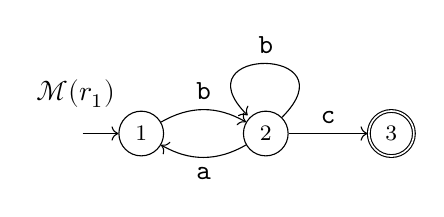
\begin{tikzpicture}
    \tikzset{
      node distance=1cm,
      every state/.append style={minimum size=0.5cm},
      initial text=$ $
    }

    \node[state, initial, label=above left:$\Automaton{r_1}$] (s0) {1};
    \node[state, right=of s0] (s1) {2};
    \node[state, accepting, right=of s1] (s2) {3};

    \draw (s0) edge[->, bend left] node[auto]{$\Char{b}$} (s1);
    \draw (s1) edge[->, bend left] node[auto]{$\Char{a}$} (s0);
    \draw (s1) edge[->, loop] node[above]{$\Char{b}$} (s1);
    \draw (s1) edge[->] node[auto]{$\Char{c}$} (s2);
  \end{tikzpicture}
\end{center}

\Ex

Vsak regularni izraz lahko ustreza večim različnim avtomatom.

\begin{gather*}
  r_2 = \Kleene{(\Char{b} \Seq (\Char{a} \Spc \Char{b})?)} \Seq \Char{c} \\
  \Automaton{r_2} = (Q_2, \Sigma, \delta_2, q_{0, 2}, F_2)
\end{gather*}

\begin{center}
  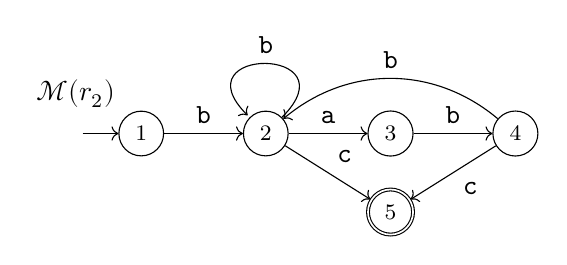
\begin{tikzpicture}
    \tikzset{
      node distance=1cm,
      every state/.append style={minimum size=0.5cm},
      initial text=$ $
    }

    \node[state, initial, label=above left:$\Automaton{r_2}$] (s0) {1};
    \node[state, right=of s0] (s1) {2};
    \node[state, right=of s1] (s2) {3};
    \node[state, right=of s2] (s3) {4};
    \node[state, accepting, below=0.4cm of s2] (s4) {5};

    \draw (s0) edge[->] node[auto]{$\Char{b}$} (s1);
    \draw (s1) edge[->, loop] node[above]{$\Char{b}$} (s1);
    \draw (s1) edge[->] node[auto]{$\Char{a}$} (s2);
    \draw (s2) edge[->] node[auto]{$\Char{b}$} (s3);
    \draw (s1) edge[->] node[auto]{$\Char{c}$} (s4);
    \draw (s3) edge[->] node[auto]{$\Char{c}$} (s4);
    \draw (s3) edge[->, bend right=40] node[above]{$\Char{b}$} (s1);
  \end{tikzpicture}
\end{center}

Funkcijo prehodov lahko definiramo tudi za niz:
\begin{align*} % XXX define empty string
  \Kleene{\delta}(q, \varepsilon) &= q\\
  \Kleene{\delta}(q, a \Seq w) &= \Kleene{\delta}(q', w) \text{, kjer } q' = \delta(q, a) \text{ in } q' \neq \Err
\end{align*}

\Ex
\begin{align*}
  \Kleene{\delta_1}(1, \Str{b}) &= 2 \\
  \Kleene{\delta_1}(1, \Str{ba}) &= 1 \\
  \Kleene{\delta_1}(1, \Str{bab}) &= 2 \\
  \Kleene{\delta_1}(1, \Str{bc}) &= 3 \\
  \Kleene{\delta_1}(1, \Str{babbc}) &= 3 \\
  \Kleene{\delta_1}(2, \Str{bbb}) &= 2 \\
  \Kleene{\delta_1}(2, \Str{abbc}) &= 3
\end{align*}

Jezik, ki ga avtomat opisuje:
\begin{equation*}
  L = \{w \in \Kleene{\Sigma} \mid \Kleene{\delta}(q_0, w) \in F\}
\end{equation*}

\Ex

\begin{align*}
  \Kleene{\delta_1}(1, \Str{bc}) &= 3 \\
  \Kleene{\delta_1}(1, \Str{bbc}) &= 3 \\
  \Kleene{\delta_1}(1, \Str{bbbc}) &= 3 \\
  \cdots \\
  \Kleene{\delta_1}(1, \Str{babc}) &= 3 \\
  \Kleene{\delta_1}(1, \Str{bababc}) &= 3 \\
  \ldots \\
  \Kleene{\delta_1}(1, \Str{babbc}) &= 3 \\
  \Kleene{\delta_1}(1, \Str{babbbc}) &= 3 \\
  \cdots \\
  \Kleene{\delta_1}(1, \Str{bababbc}) &= 3 \\
  \Kleene{\delta_1}(1, \Str{bababbbc}) &= 3 \\
  \cdots \\
\end{align*}

\begin{multline*}
  L = \{ \Str{bc}, \Str{bbc}, \Str{bbbc}, \ldots, \Str{babc}, \Str{bababc}, \ldots,\\
  \Str{babbc},  \Str{babbbc}, \ldots, \Str{bababbc}, \Str{bababbbc}, \dots \}
\end{multline*}

Za implementacijo pregledovalnika je potrebno končnemu avtomatu dodati funkcijo, ki končna stanja preslika v terminale:
\begin{equation*}
  \acc: Q \rightarrow T
\end{equation*}

\section{Konstrukcija}

\Special{Meta:} Jezik regularnega izraza $r$ bo označen kot $\Language{r}$.\\

Regularni izraz v končni avtomat pretvorimo tako, da najprej ustvarimo končne avtomate za posamezne elemente $\Char{a}$, $\Empty$, $\Null$, ki jih nato s pomočjo pravil za konstrukcijo združujemo.

%Pri opisani konstrukciji so vsi prehodi, ki vodijo v katero koli stanje stanje označeni z enakim znakom.
%\begin{center}
%  \begin{tikzpicture}
%    \tikzset{
%      ->,
%      node distance=1cm,
%      every state/.append style={minimum size=0.5cm},
%      initial text=$ $
%    }
%
%
%    \node[state] (s) {};
%
%    \node[left=1 of s] (i1) {$\ldots$};
%    \node[above left=1 of s] (i2) {$\ddots$};
%    \node[below left=1 of s] (i3) {\reflectbox{$\ddots$}};
%    \draw(i1) edge node[auto]{\Char{a}} (s);
%    \draw(i2) edge node[auto]{\Char{a}} (s);
%    \draw(i3) edge node[auto]{\Char{a}} (s);
%
%  \end{tikzpicture}
%\end{center}
%To je posebna lastnost končnih avtomat ustvarjenih s to konstrukcijo in ne velja za poljuben končni avtomat.

Sledijo definicije in pravila za konstrucijo za vse operacije in elemente.

\subsection{Prazen jezik}
\begin{tcolorbox}[title={Definicija}]
\begin{equation*}
  \begin{aligned}
    r &= \Empty\\
    \Language{r} &= \{\}
  \end{aligned}
\end{equation*}
\end{tcolorbox}

\begin{center}
  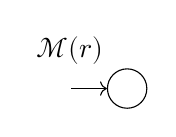
\begin{tikzpicture}
    \tikzset{
      ->,
      node distance=1cm,
      every state/.append style={minimum size=0.5cm},
      initial text=$ $
    }

    \node[state, initial, label=above left:$\Automaton{r}$] {};
  \end{tikzpicture}
\end{center}


\subsection{Prazen niz}

\begin{tcolorbox}[title={Definicija}]
\begin{equation*}
  \begin{aligned}
    r &= \Null\\
    \Language{r} &= \{ \Str{} \}
  \end{aligned}
\end{equation*}
\end{tcolorbox}

\begin{center}
  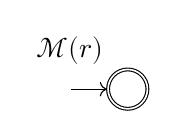
\begin{tikzpicture}
    \tikzset{
      ->,
      node distance=1cm,
      every state/.append style={minimum size=0.5cm},
      initial text=$ $
    }

    \node[state, initial, accepting, label=above left:$\Automaton{r}$] {};
  \end{tikzpicture}
\end{center}

Če $\Str{} \in \Language{r}$, potem rečemo, da je $r$ \emph{nullable}.

\subsection{Znak}

\begin{tcolorbox}[title={Definicija}]
\begin{equation*}
  \begin{aligned}
    r &= \Char{a}\text{, kjer } \Char{a} \in \Alphabet\\\
    \Language{r} &= \{ \Str{a} \}
  \end{aligned}
\end{equation*}
\end{tcolorbox}

\begin{center}
  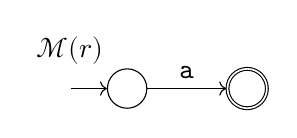
\begin{tikzpicture}
    \tikzset{
      ->,
      node distance=1cm,
      every state/.append style={minimum size=0.5cm},
      initial text=$ $
    }

    \node[state, initial, label=above left:$\Automaton{r}$] (q0) {};
    \node[state, accepting, right=of q0] (q1) {};

    \draw (q0) edge node[auto]{$\Char{a}$} (q1);
  \end{tikzpicture}
\end{center}

\subsection{Množica znakov}
\Reset

\begin{tcolorbox}[title={Definicija}]
\begin{equation*}
  \begin{aligned}
    r &= S\text{, kjer } S \subseteq \Alphabet \\
    &= \Char{a} \Union \dots \Union \Char{b}\text{, kjer } \Char{a}, \dots, \Char{b} \in S\\
    \Language{r} &= S
  \end{aligned}
\end{equation*}
\end{tcolorbox}

\Ex
\begin{equation*}
  \begin{aligned}
    \N{r} &= \{ \Char{a}, \Char{b}, \Char{c} \} \\
    \N{r} &= \Char{a} \Union \Char{b} \Union \Char{c}
  \end{aligned}
\end{equation*}

Množica znakov se lahko predstavi kot šop robov (eden za vsak znak) ali pa en sam rob označen z množico.
\begin{center}
  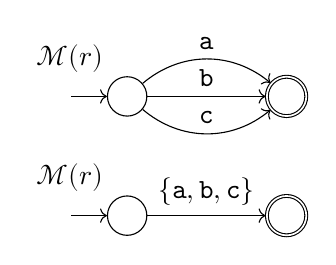
\begin{tikzpicture}
    \tikzset{
      ->,
      node distance=1cm,
      every state/.append style={minimum size=0.5cm},
      initial text=$ $
    }

    \node[state, initial, label=above left:$\Automaton{\N{r}}$] (p0) {};
    \node[state, accepting, right=1.5cm of p0] (p1) {};

    \node[state, initial, below=of p0, label=above left:$\Automaton{\N{r}}$] (q0) {};
    \node[state, accepting, right=1.5cm of q0] (q1) {};


    \draw (q0) edge node[auto]{$\{\Char{a}, \Char{b}, \Char{c} \} $} (q1);

    \draw (p0) edge[bend left=40] node[auto]{$\Char{a}$} (p1);
    \draw (p0) edge node[auto]{$\Char{b}$} (p1);
    \draw (p0) edge[bend right=40] node[auto]{$\Char{c}$} (p1);
  \end{tikzpicture}
\end{center}
\Next

\subsection*{Primeri}

\subsubsection{Y/N}

\begin{equation*}
  \Language{\N{r}} = \{ \Str{Y}, \Str{N} \}
\end{equation*}

\begin{equation*}
  \N{r} = \{ \Char{Y}, \Char{N} \}
\end{equation*}

\begin{center}
  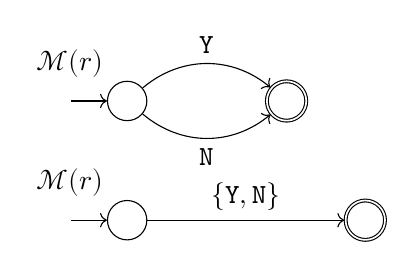
\begin{tikzpicture}
    \tikzset{
      ->,
      node distance=1cm,
      every state/.append style={minimum size=0.5cm},
      initial text=$ $
    }

    \node[state, initial, label=above left:$\Automaton{\N{r}}$] (p0) {};
    \node[state, accepting, right=1.5cm of p0] (p1) {};

    \node[state, initial, below=of p0, label=above left:$\Automaton{\N{r}}$] (q0) {};
    \node[state, accepting, right=2.5cm of q0] (q1) {};


    \draw (q0) edge node[auto]{$\{\Char{Y}, \Char{N} \} $} (q1);

    \draw (p0) edge[bend left=40] node[auto]{$\Char{Y}$} (p1);
    \draw (p0) edge[bend right=40] node[below]{$\Char{N}$} (p1);
  \end{tikzpicture}
\end{center}
\Next

\subsubsection{Števke}

\begin{equation*}
  \Language{\N{r}} = \{ \Str{0}, \Str{1}, \Str{2}, \dots, \Str{9} \}
\end{equation*}

\begin{equation*}
  \N{r} = \{ \Char{0}, \Char{1}, \Char{2}, \dots, \Char{9} \}
\end{equation*}

\begin{center}
  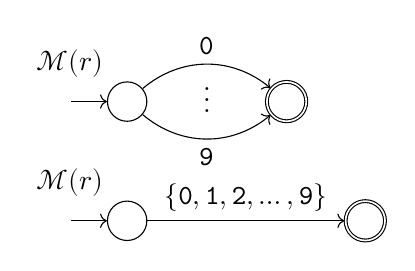
\begin{tikzpicture}
    \tikzset{
      ->,
      node distance=1cm,
      every state/.append style={minimum size=0.5cm},
      initial text=$ $
    }

    \node[state, initial, label=above left:$\Automaton{\N{r}}$] (p0) {};
    \node[state, accepting, right=1.5cm of p0] (p1) {};
    \node at ($(p0)!0.5!(p1)$) {\Dots{}};

    \node[state, initial, below=of p0, label=above left:$\Automaton{\N{r}}$] (q0) {};
    \node[state, accepting, right=2.5cm of q0] (q1) {};


    \draw (q0) edge node[auto]{$\{\Char{0}, \Char{1}, \Char{2}, \ldots, \Char{9} \} $} (q1);

    \draw (p0) edge[bend left=40] node[auto]{$\Char{0}$} (p1);
    \draw (p0) edge[bend right=40] node[below]{$\Char{9}$} (p1);
  \end{tikzpicture}
\end{center}
\Next

\subsubsection{Male črke}

\begin{equation*}
  \Language{\N{r}} = \{ \Str{a}, \Str{b}, \Str{c}, \dots, \Str{z} \}
\end{equation*}
\Next

\subsubsection{Velike in male črke}

\begin{equation*}
  \Language{\N{r}} = \{ \Str{A}, \Str{B}, \Str{C}, \dots, \Str{Z}, \Str{a}, \Str{b}, \Str{c}, \dots, \Str{z} \}
\end{equation*}
\Next

\subsubsection{Heksadecimalne števke}

\begin{equation*}
  \Language{\N{r}} = \{ \Str{0}, \Str{1}, \Str{2}, \dots, \Str{9}, \Str{A}, \dots, \Str{F} \}
\end{equation*}
\Next

\newpage
\subsection{Konkatenacija}
\Reset

\begin{tcolorbox}[title={Definicija}]
\begin{equation*}
  \begin{aligned}
  r &= s \Seq t = s \Spc t\\
  \Language{r} &= \{ u \Seq v \mid u \in \Language{s} \land v \in \Language{t}\}
  \end{aligned}
\end{equation*}
\end{tcolorbox}

\begin{tcolorbox}[title={Pravila}]
\begin{equation*}
  \begin{aligned}
  s \Seq t &\not= t \Seq s\\
  s \Seq \Null &= s \\
  \Null \Seq s &= s   \\
  s \Seq \Empty &= \Empty \\
  \Empty \Seq s &= \Empty \\
  (s \Seq p) \Seq q &= s \Seq (p \Seq q) = s \Seq p \Seq q
  \end{aligned}
\end{equation*}
\end{tcolorbox}

\vspace{1em}
\Special{Poseben primer:} Če $|\Language{s}| = |\Language{t}| = 1$, potem $\Language{s} = \{u\}$ in $\Language{t} = \{v\}$ in $\Language{r} = \{u \Seq v\}$.

\Ex
\begin{align*}
  \Language{s} &= \{\Str{Hello}\}\\
  \Language{t} &= \{\Str{World}\}\\
  \Language{r} &= \{\Str{HelloWorld}\}
\end{align*}

Splošno je jezik konkatenacije podoben kartezičnemu produktu.
\begin{align*}
  S &= P \times Q \\
  S &= \{ (x, y) \mid x \in P \land y \in Q\}
\end{align*}

\Ex
\begin{align*}
  P &= \{1, 2, 3\}\\
  Q &= \{a, b\}\\
  S &= \{(1, a), (1, b), (2, a), (2, b), (3, a), (3, b) \}
\end{align*}

Edina razlika je da zamenjamo vsak $(u, v)$, kjer $u \in \Language{s}$ in $v\in \Language{t}$, z $u \Seq v \in \Language{r}$.

\Ex

\begin{align*}
  P &= \{\Str{Dober}, \Str{Lep}\}\\
  Q &= \{\Str{Dan}, \Str{Večer}, \Str{Tek}\}\\
  S &= \{\Str{DoberDan}, \Str{DoberVečer}, \Str{DoberTek}, \Str{LepDan}, \Str{LepVečer}, \Str{LepTek} \}
\end{align*}

Končni avtomat konkatenacije $\Automaton{r}$ dveh končnih avtomatov $\Automaton{s}$ in $\Automaton{t}$ sestavimo tako:
\begin{enumerate}
  \item Ustvarimo prehod $\delta(q, \Char{a}) = q'$ iz vsakega končnega stanja $q$ v $\Automaton{s}$ v vsako stanje $q'$, ki je direktno dosegljivo iz začetnega stanja v $\Automaton{t}$ (vsakega z vsakim). 
    Ustvarjen prehod je označen z enakim simbolom $\Char{a}$, kot obstoječi prehod, ki vodi iz začetnega stanja v $q'$.
  \item Začetno stanje $\Automaton{t}$ odstranimo.
  \item Končna stanja $\Automaton{s}$ označimo kot ne-končna, razen če je končno začetno stanje $\Automaton{t}$.
\end{enumerate}

\begin{center}
  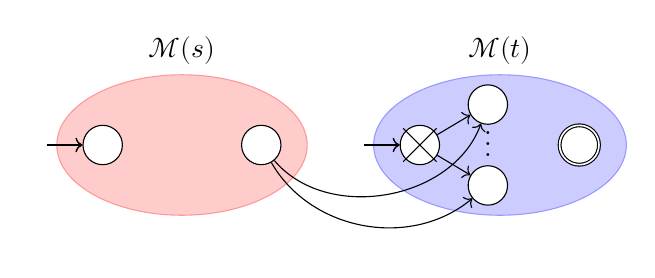
\begin{tikzpicture}
    \tikzset{
      node distance=1cm,
      every state/.append style={fill=white, minimum size=0.5cm},
      initial text=$ $
    }

    \node[initial, state, initial] (s0) {};
    \node[state, hide, above right=0.15cm and 0.5cm of s0] (s1) {};
    \node[state, hide, fill=none, below right=0.15cm and 0.5cm of s0] (s2) {};
    \node[state, right=1.5cm of s0] (sn) {};

    \begin{pgfonlayer}{background}
      \node[fit=(s0) (s1) (s2) (sn), draw=red!40, fill=red!20, ellip, label=above:$\Automaton{s}$] (qm) {};
    \end{pgfonlayer}

    \node[initial, state, initial, right=1.5cm of sn] (p0) {};
    \path (p0) pic {cross=0.30cm};
    \node[state, above right=0.15cm and 0.5cm of p0] (p1) {};
    \node[state, below right=0.15cm and 0.5cm of p0] (p2) {};
    \node at ($(p1)!0.5!(p2)$) {\Dots{}};
    \draw (p0) edge[->] (p1);
    \draw (p0) edge[->] (p2);
    \draw (sn) edge[->, bend right=60] (p1);
    \draw (sn) edge[->, bend right=50] (p2);
    \node[state, accepting, right=1.5cm of p0] (pn) {};

    \begin{pgfonlayer}{background}
      \node[fit=(p0) (p1) (p2) (pn), ellip, draw=blue!40, fill=blue!20, label=above:$\Automaton{t}$] (pm) {};
    \end{pgfonlayer}
  \end{tikzpicture}
\end{center}

\Ex
\begin{align*}
  \N{s} &= \Char{a} \\
  \N{t} &= \Char{b} \\
  \N{r} &= \Char{a} \Spc \Char{b} \\
\end{align*}

\begin{align*}
  \Language{\N{s}} &= \{\Str{a}\} \\
  \Language{\N{t}} &= \{\Str{b}\} \\
  \Language{\N{r}} &= \{\Str{ab}\}
\end{align*}

\begin{center}
  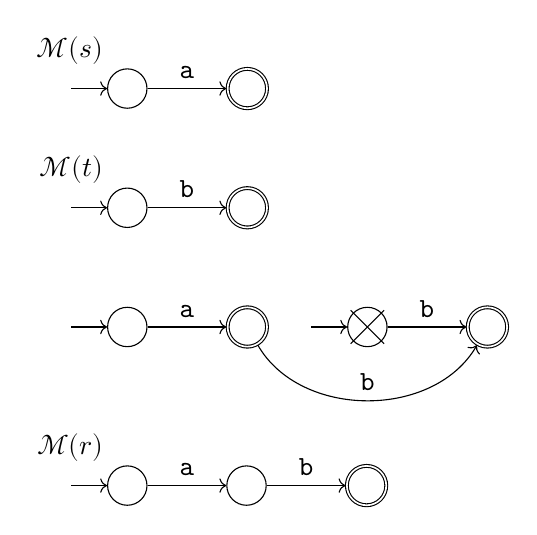
\begin{tikzpicture}
    \tikzset{
      node distance=1cm,
      every state/.append style={minimum size=0.5cm},
      initial text=$ $
    }

    \node[state, initial, label=above left:$\Automaton{\N{s}}$] (x0) {};
    \node[state, accepting, right=of x0] (x1) {};

    \draw (x0) edge[->] node[auto]{$\Char{a}$} (x1);

    \node[state, initial, label=above left:$\Automaton{\N{t}}$, below=of x0] (y0) {};
    \node[state, accepting, right=of y0] (y1) {};

    \draw (y0) edge[->] node[auto]{$\Char{b}$} (y1);

    \node[state, initial, below=of y0] (q0) {};
    \node[state, accepting, right=of q0] (q1) {};

    \draw (q0) edge[->] node[auto]{$\Char{a}$} (q1);

    \node[state, initial, right=of q1] (p0) {};
    \path (p0) pic {cross=0.30cm};
    \node[state, accepting, right=of p0] (p1) {};

    \draw (p0) edge[->] node[auto]{$\Char{b}$} (p1);

    \draw (q1) edge[->, bend right=60] node[auto]{$\Char{b}$} (p1);

    \node[state, initial, label=above left:$\Automaton{\N{r}}$, below=1.5cm of q0] (s0) {};
    \node[state, right=of s0] (s1) {};
    \node[state, accepting, right=of s1] (s2) {};

    \draw (s0) edge[->] node[auto]{$\Char{a}$} (s1);
    \draw (s1) edge[->] node[auto]{$\Char{b}$} (s2);
  \end{tikzpicture}
\end{center}
\Next

\Ex

\begin{align*}
  \N{s} &= \Char{a} \Spc \Char{b} \\
  \N{t} &= \Char{c} \\
  \N{r} &= \Char{a} \Spc \Char{b} \Spc \Char{c} \\
\end{align*}

\begin{align*}
  \Language{\N{s}} &= \{\Str{ab}\} \\
  \Language{\N{t}} &= \{\Str{c}\} \\
  \Language{\N{r}} &= \{\Str{abc}\}
\end{align*}

\begin{center}
  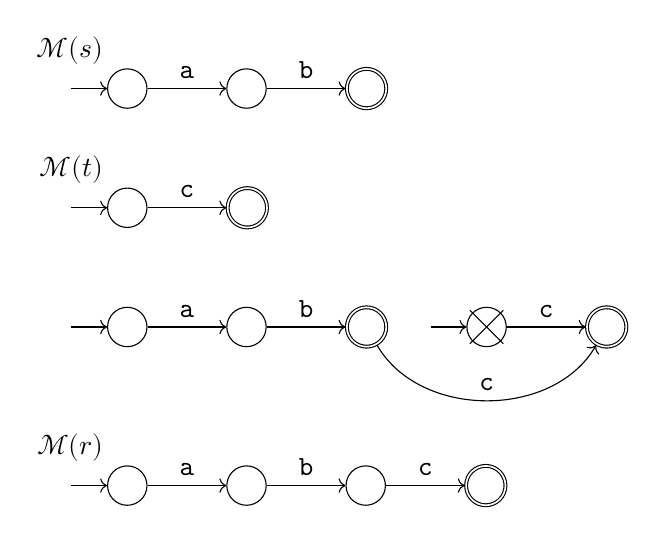
\begin{tikzpicture}
    \tikzset{
      node distance=1cm,
      every state/.append style={minimum size=0.5cm},
      initial text=$ $
    }

    \node[state, initial, label=above left:$\Automaton{\N{s}}$] (x0) {};
    \node[state, right=of x0] (x1) {};
    \node[state, accepting, right=of x1] (x2) {};

    \draw (x0) edge[->] node[auto]{$\Char{a}$} (x1);
    \draw (x1) edge[->] node[auto]{$\Char{b}$} (x2);

    \node[state, initial, label=above left:$\Automaton{\N{t}}$, below=of x0] (y0) {};
    \node[state, accepting, right=of y0] (y1) {};

    \draw (y0) edge[->] node[auto]{$\Char{c}$} (y1);

    \node[state, initial, below=of y0] (q0) {};
    \node[state, right=of q0] (q1) {};
    \node[state, accepting, right=of q1] (q2) {};

    \draw (q0) edge[->] node[auto]{$\Char{a}$} (q1);
    \draw (q1) edge[->] node[auto]{$\Char{b}$} (q2);

    \node[state, initial, right=of q2] (p0) {};
    \path (p0) pic {cross=0.30cm};
    \node[state, accepting, right=of p0] (p1) {};

    \draw (p0) edge[->] node[auto]{$\Char{c}$} (p1);

    \draw (q2) edge[->, bend right=60] node[auto]{$\Char{c}$} (p1);

    \node[state, initial, label=above left:$\Automaton{\N{r}}$, below=1.5cm of q0] (s0) {};
    \node[state, right=of s0] (s1) {};
    \node[state, right=of s1] (s2) {};
    \node[state, accepting, right=of s2] (s3) {};

    \draw (s0) edge[->] node[auto]{$\Char{a}$} (s1);
    \draw (s1) edge[->] node[auto]{$\Char{b}$} (s2);
    \draw (s2) edge[->] node[auto]{$\Char{c}$} (s3);
  \end{tikzpicture}
\end{center}
\Next

\Ex
\begin{align*}
  \N{s} &= \Char{a} \Spc \Char{b} \\
  \N{t} &= \Char{c} \Spc \Char{d} \\
  \N{r} &= \Char{a} \Spc \Char{b} \Spc \Char{c} \Spc \Char{d} \\
\end{align*}

\begin{align*}
  \Language{\N{s}} &= \{\Str{ab}\} \\
  \Language{\N{t}} &= \{\Str{cd}\} \\
  \Language{\N{r}} &= \{\Str{abcd}\}
\end{align*}

\begin{center}
  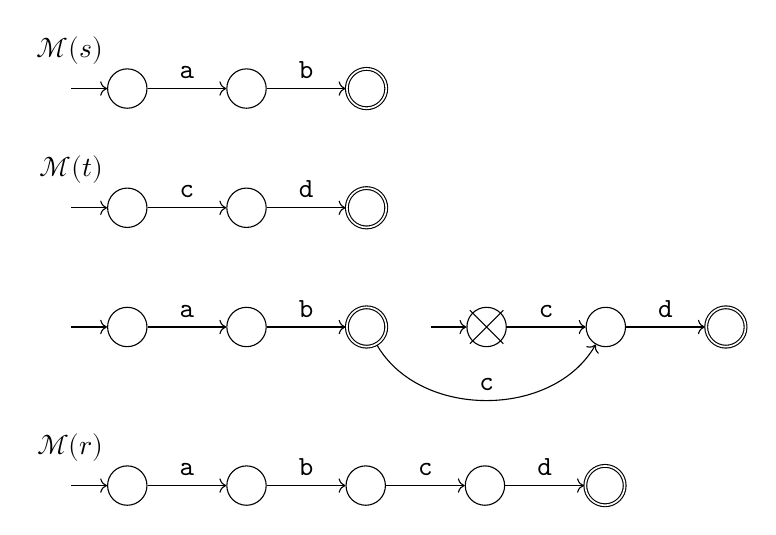
\begin{tikzpicture}
    \tikzset{
      node distance=1cm,
      every state/.append style={minimum size=0.5cm},
      initial text=$ $
    }

    \node[state, initial, label=above left:$\Automaton{\N{s}}$] (x0) {};
    \node[state, right=of x0] (x1) {};
    \node[state, accepting, right=of x1] (x2) {};

    \draw (x0) edge[->] node[auto]{$\Char{a}$} (x1);
    \draw (x1) edge[->] node[auto]{$\Char{b}$} (x2);

    \node[state, initial, label=above left:$\Automaton{\N{t}}$, below=of x0] (y0) {};
    \node[state, right=of y0] (y1) {};
    \node[state, accepting, right=of y1] (y2) {};

    \draw (y0) edge[->] node[auto]{$\Char{c}$} (y1);
    \draw (y1) edge[->] node[auto]{$\Char{d}$} (y2);

    \node[state, initial, below=of y0] (q0) {};
    \node[state, right=of q0] (q1) {};
    \node[state, accepting, right=of q1] (q2) {};

    \draw (q0) edge[->] node[auto]{$\Char{a}$} (q1);
    \draw (q1) edge[->] node[auto]{$\Char{b}$} (q2);

    \node[state, initial, right=of q2] (p0) {};
    \path (p0) pic {cross=0.30cm};
    \node[state, right=of p0] (p1) {};
    \node[state, accepting, right=of p1] (p2) {};

    \draw (p0) edge[->] node[auto]{$\Char{c}$} (p1);
    \draw (p1) edge[->] node[auto]{$\Char{d}$} (p2);

    \draw (q2) edge[->, bend right=60] node[auto]{$\Char{c}$} (p1);

    \node[state, initial, label=above left:$\Automaton{\N{r}}$, below=1.5cm of q0] (s0) {};
    \node[state, right=of s0] (s1) {};
    \node[state, right=of s1] (s2) {};
    \node[state, right=of s2] (s3) {};
    \node[state, accepting, right=of s3] (s4) {};

    \draw (s0) edge[->] node[auto]{$\Char{a}$} (s1);
    \draw (s1) edge[->] node[auto]{$\Char{b}$} (s2);
    \draw (s2) edge[->] node[auto]{$\Char{c}$} (s3);
    \draw (s3) edge[->] node[auto]{$\Char{d}$} (s4);
  \end{tikzpicture}
\end{center}
\Next

\subsection*{Primeri}

\subsubsection{"then"}
\begin{equation*}
  \Language{\N{r}} = \{ \Str{then} \}
\end{equation*}
\Next

\subsubsection{"then", "Then", "THEN", "theN", ...}
Če so robovi avtomatov označeni z množico znakov, avtomat konkatenacije sestavimo na čisto enak način, kot če bi bil na robovih en sam znak.
\begin{equation*}
  \N{r} = \{\Char{T}, \Char{t}\} \Seq \{\Char{H}, \Char{h}\} \Seq \{\Char{E}, \Char{e}\} \Seq \{\Char{N}, \Char{n}\}
\end{equation*}

\Next
\subsubsection{Bajt po osmiško}

\begin{equation*}
  \N{r} = \{\Char{0}, \dots, \Char{3}\} \Seq \{\Char{0}, \dots, \Char{7}\} \Seq \{\Char{0}, \dots, \Char{7}\}
\end{equation*}

\begin{equation*}
  \Language{\N{r}} = \{ \Str{000}, \Str{001}, \Str{002}, \dots, \Str{377} \}
\end{equation*}
\Next

\subsection{Potence}
\Reset

\begin{tcolorbox}[title={Definicija}]
\begin{equation*}
  \begin{aligned}
    \Rep{s}{0} &= \Null\\
    \Rep{s}{i+1} &= \Rep{s}{i} \Seq s\\[1em]
    \Rep{s}{i} &= \underbrace{s \Seq \ldots \Seq s}_{i}\\[1em]
    \Language{\Rep{s}{0}} &= \Null\\
    \Language{\Rep{s}{i+1}} &= \{u \Seq v \mid u \in \Language{\Rep{s}{i}} \land v \in \Language{s}\}
  \end{aligned}
\end{equation*}
\end{tcolorbox}
\begin{align*}
\end{align*}

Avtomat $\Automaton{\Rep{s}{i}}$ sestavimo tako, da konkateniramo $i$ kopij avtomata $\Automaton{s}$.
Avtomat $\Automaton{\Rep{s}{0}}$ je enak, kot avtomat za prazen niz.

\begin{center}
  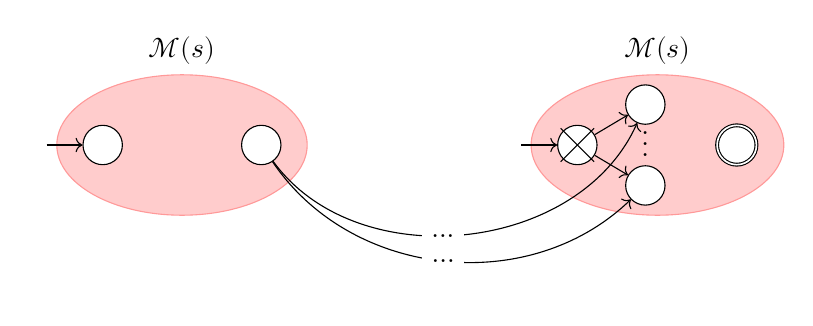
\begin{tikzpicture}
    \tikzset{
      node distance=1cm,
      every state/.append style={fill=white, minimum size=0.5cm},
      initial text=$ $
    }

    \node[state, initial] (s0) {};
    \node[state, hide, above right=0.15cm and 0.5cm of s0] (s1) {};
    \node[state, hide, below right=0.15cm and 0.5cm of s0] (s2) {};
    \node[state, right=1.5cm of s0] (sn) {};

    \begin{pgfonlayer}{background}
      \node[fit=(s0) (s1) (s2) (sn), ellip, draw=red!40, fill=red!20, label=above:$\Automaton{s}$] (qm) {};
    \end{pgfonlayer}

    \node[state, initial, right=3.5cm of sn] (p0) {};
    \path (p0) pic {cross=0.30cm};
    \node[state, above right=0.15cm and 0.5cm of p0] (p1) {};
    \node[state, below right=0.15cm and 0.5cm of p0] (p2) {};
    \node at ($(p1)!0.5!(p2)$) {\Dots{}};
    \draw (p0) edge[->] (p1);
    \draw (p0) edge[->] (p2);
    \draw (sn) edge[->, bend right=60] node[pos=0.45,fill=white] {...} (p1);
    \draw (sn) edge[->, bend right=50] node[pos=0.5,fill=white] {...} (p2);
    \node[state, accepting, right=1.5cm of p0] (pn) {};

    \begin{pgfonlayer}{background}
      \node[fit=(p0) (p1) (p2) (pn), ellip, draw=red!40, fill=red!20, label=above:$\Automaton{s}$] (pm) {};
    \end{pgfonlayer}
  \end{tikzpicture}
\end{center}

\subsection*{Primeri}

\subsubsection{"aaaa"}

\begin{align*}
  \N{s} &= \Char{a} \\
  \N{r} &= \Char{a}^4
\end{align*}

\begin{align*}
  \Language{\N{s}} &= \{\Str{a}\} \\
  \Language{\N{r}} &= \{\Str{aaaa}\} \\
\end{align*}
\Next

\subsubsection{"abab"}

\begin{align*}
  \N{s} &= \Char{a} \Spc \Char{b} \\
  \N{r} &= (\Char{a} \Spc \Char{b})^2
\end{align*}

\begin{align*}
  \Language{\N{s}} &= \{\Str{ab}\} \\
  \Language{\N{r}} &= \{\Str{abab}\} \\
\end{align*}
\Next

\subsubsection{Bajt po osmiško}
\begin{equation*}
  \N{r} = \{\Char{0}, \dots, \Char{3}\} \Seq (\{\Char{0}, \dots, \Char{7}\})^2
\end{equation*}
\Next

\subsection{Unija}
\Reset

\begin{tcolorbox}[title={Definicija}]
  \begin{equation*}
    \begin{aligned}
    r &= s \Union t \\
      \Language{r} &= \Language{s} \cup \Language{t}
    \end{aligned}
  \end{equation*}
\end{tcolorbox}

\begin{tcolorbox}[title={Pravila}]
  \begin{equation*}
    \begin{aligned}
      s \Union t &= t \Union s \\
      s \Union s &= s \\
      \Empty \Union s &= s \\
      s \Union \Empty &= s \\
      (s \Union p) \Union q &= s \Union (p \Union q) = s \Union p \Union q \\
      s \Seq (p \Union q) &= s \Seq p \Union s \Seq q\\
      (p \Union q) \Seq s &= p \Seq s \Union q \Seq s\\
    \end{aligned}
  \end{equation*}
\end{tcolorbox}

Končni avtomat unije $\Automaton{r}$ dveh končnih avtomatov $\Automaton{s}$ in $\Automaton{t}$ sestavimo tako:
\begin{enumerate}
\item Ustvarimo novo začetno stanje $q$.

\item Ustvarimo prehod $\delta(q, \Char{a}) = q'$ iz novega začetnega stanja $q$ v vsako stanje $q'$, ki je direktno dosegljivo iz začetnega stanja v $\Automaton{s}$ ali $\Automaton{t}$.
    Ustvarjen prehod je označen z enakim simbolom $\Char{a}$, kot obstoječi prehod, ki vodi iz začetnega stanja v $q'$.
\item Začetni stanji $\Automaton{s}$ in $\Automaton{t}$ odstranimo.
\item Začetno stanje $\Automaton{r}$ je končno če je končno začetno stanje $\Automaton{s}$ ali $\Automaton{t}$.
\end{enumerate}

\begin{center}
  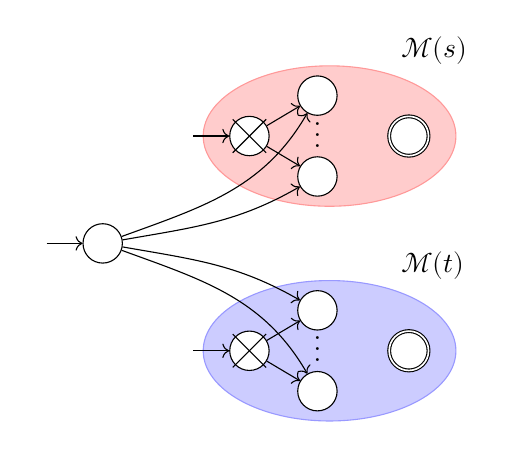
\begin{tikzpicture}
    \tikzset{
      node distance=1cm,
      every state/.append style={fill=white, minimum size=0.5cm},
      initial text=$ $
    }

    \node[state, initial] (q0) {};

    \node[state, above right=1.0cm and 1.5cm of q0, initial] (s0) {};
    \path (s0) pic {cross=0.30cm};
    \node[state, above right=0.15cm and 0.5cm of s0] (s1) {};
    \node[state, below right=0.15cm and 0.5cm of s0] (s2) {};
    \node at ($(s1)!0.5!(s2)$) {\Dots{}};
    \draw (s0) edge[->] (s1);
    \draw (s0) edge[->] (s2);
    \draw (q0) edge[->, out=20+0, in=-120] (s1);
    \draw (q0) edge[->, out=10+0, in=-150+0] (s2);
    \node[state, accepting, right=1.5cm of s0] (sn) {};

    \begin{pgfonlayer}{background}
      \node[fit=(s0) (s1) (s2) (sn), ellip, draw=red!40, fill=red!20, label=above right:$\Automaton{s}$] (qm) {};
    \end{pgfonlayer}

    \node[state, below right=1.0cm and 1.5cm of q0, initial] (p0) {};
    \path (p0) pic {cross=0.30cm};
    \node[state, above right=0.15cm and 0.5cm of p0] (p1) {};
    \node[state, below right=0.15cm and 0.5cm of p0] (p2) {};
    \node at ($(p1)!0.5!(p2)$) {\Dots{}};
    \draw (p0) edge[->] (p1);
    \draw (p0) edge[->] (p2);
    \draw (q0) edge[->, out=-10+0, in=150+0] (p1);
    \draw (q0) edge[->, out=-20+0, in=120] (p2);
    \node[state, accepting, right=1.5cm of p0] (pn) {};

    \begin{pgfonlayer}{background}
      \node[fit=(p0) (p1) (p2) (pn), ellip, draw=blue!40, fill=blue!20, label=above right:$\Automaton{t}$] (pm) {};
    \end{pgfonlayer}
  \end{tikzpicture}
\end{center}

\Ex
\begin{align*}
  \N{s} &= \Char{a} \\
  \N{t} &= \Char{b} \\
  \N{r} &= \Char{a} \Union \Char{b}
\end{align*}

\begin{align*}
  \Language{\N{s}} &= \{\Str{a}\} \\
  \Language{\N{t}} &= \{\Str{b}\} \\
  \Language{\N{r}} &= \{\Str{a}, \Str{b}\} \\
\end{align*}

\begin{center}
  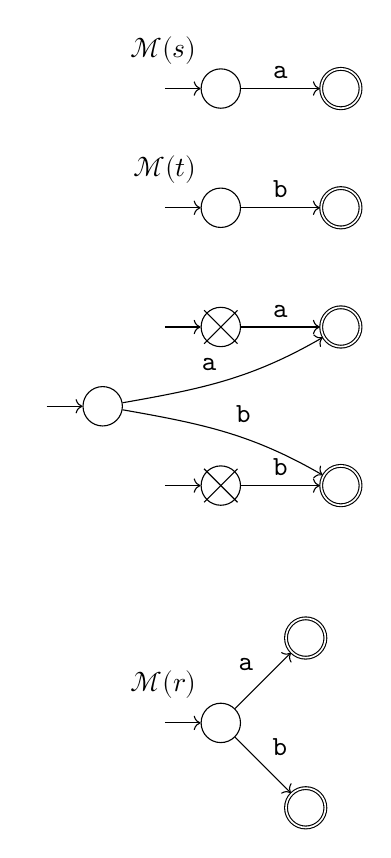
\begin{tikzpicture}
    \tikzset{
      node distance=1cm,
      every state/.append style={minimum size=0.5cm},
      initial text=$ $
    }

    \node[state, initial, label=above left:$\Automaton{\N{s}}$] (x0) {};
    \node[state, accepting, right=of x0] (x1) {};

    \draw (x0) edge[->] node[auto]{$\Char{a}$} (x1);

    \node[state, initial, label=above left:$\Automaton{\N{t}}$, below=of x0] (y0) {};
    \node[state, accepting, right=of y0] (y1) {};

    \draw (y0) edge[->] node[auto]{$\Char{b}$} (y1);

    \node[state, initial, below=of y0] (q0) {};
    \path (q0) pic {cross=0.30cm};
    \node[state, accepting, right=of q0] (q1) {};

    \draw (q0) edge[->] node[auto]{$\Char{a}$} (q1);

    \node[state, initial, below=1.5cm of q0] (p0) {};
    \path (p0) pic {cross=0.30cm};
    \node[state, accepting, right=of p0] (p1) {};

    \draw (p0) edge[->] node[auto]{$\Char{b}$} (p1);

    \node[state, initial] at ($(q0)!0.5!(p0) - (1.5, 0)$) (n) {};

    \draw (n) edge[->, out=10+0, in=-150+0] node[auto] {$\Char{a}$} (q1);
    \draw (n) edge[->, out=-10+0, in=150+0] node[auto] {$\Char{b}$} (p1);

    \node[state, initial, below=2.5cm of p0, label=above left:$\Automaton{\N{r}}$] (u0) {};
    \node[state, accepting, above right=of u0] (u1) {};

    \draw (u0) edge[->] node[auto]{$\Char{a}$} (u1);

    \node[state, accepting, below right=of u0] (u4) {};

    \draw (u0) edge[->] node[auto]{$\Char{b}$} (u4);

  \end{tikzpicture}
\end{center}
\Next

\Ex
\begin{align*}
  \N{s} &= \Char{a} \Union \Char{b} \\
  \N{t} &= \Char{c} \Union \Char{d} \\
  \N{r} &= (\Char{a} \Union \Char{b}) \Seq (\Char{c} \Union \Char{d})
\end{align*}

\begin{align*}
  \Language{\N{s}} &= \{\Str{a}, \Str{b}\} \\
  \Language{\N{t}} &= \{\Str{c}, \Str{d}\} \\
  \Language{\N{r}} &= \{\Str{ac}, \Str{ad}, \Str{bc}, \Str{bd}\} \\
\end{align*}

\begin{center}
  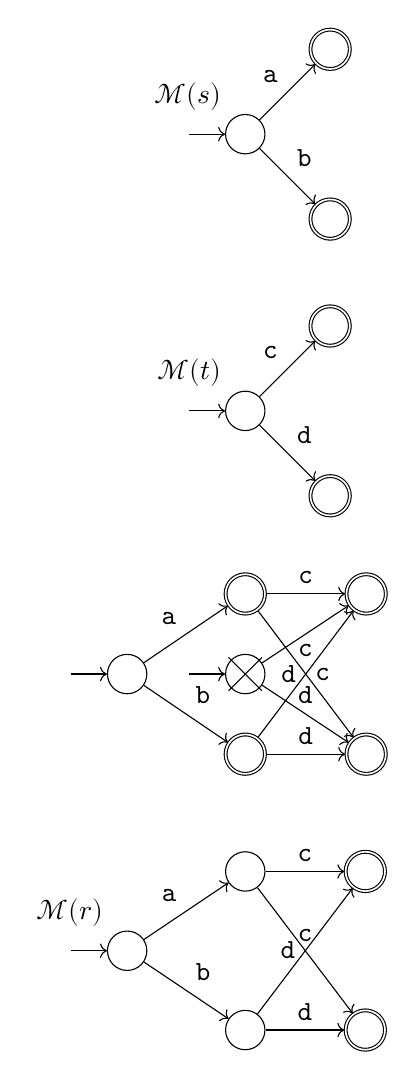
\begin{tikzpicture}
    \tikzset{
      node distance=1cm,
      every state/.append style={minimum size=0.5cm},
      initial text=$ $
    }

    \node[state, initial, label=above left:$\Automaton{\N{s}}$] (x0) {};
    \node[state, accepting, above right=of x0] (x1) {};
    \node[state, accepting, below right=of x0] (x2) {};

    \draw (x0) edge[->] node[auto]{$\Char{a}$} (x1);
    \draw (x0) edge[->] node[auto]{$\Char{b}$} (x2);

    \node[state, initial, label=above left:$\Automaton{\N{t}}$, below=3 of x0] (y0) {};
    \node[state, accepting, above right=of y0] (y1) {};
    \node[state, accepting, below right=of y0] (y2) {};

    \draw (y0) edge[->] node[auto]{$\Char{c}$} (y1);
    \draw (y0) edge[->] node[auto]{$\Char{d}$} (y2);

    \node[state, accepting, below=1.8 of y0] (q0) {};
    \node[state, accepting, right=of q0] (q1) {};

    \draw (q0) edge[->] node[auto]{$\Char{c}$} (q1);

    \node[state, accepting, below=1.5cm of q0] (p0) {};
    \node[state, accepting, right=of p0] (p1) {};

    \draw (p0) edge[->] node[auto]{$\Char{d}$} (p1);

    \node[state, initial] at ($(q0)!0.5!(p0) - (1.5, 0)$) (n) {};

    \node[state, initial] at ($(q0)!0.5!(p0)$) (n1) {};
    \path (n1) pic {cross=0.30cm};

    \draw (n) edge[->] node[auto] {$\Char{a}$} (q0);
    \draw (n) edge[->] node[auto] {$\Char{b}$} (p0);

    \draw (n1) edge[->] node[below] {$\Char{c}$} (q1);
    \draw (n1) edge[->] node[above] {$\Char{d}$} (p1);

    \draw (p0) edge[->] node[right] {$\Char{c}$} (q1);
    \draw (q0) edge[->] node[left] {$\Char{d}$} (p1);

    \node[state, below=3.0 of q0] (e0) {};
    \node[state, accepting, right=of e0] (e1) {};

    \draw (e0) edge[->] node[auto]{$\Char{c}$} (e1);

    \node[state, below=1.5cm of e0] (f0) {};
    \node[state, accepting, right=of f0] (f1) {};

    \draw (f0) edge[->] node[auto]{$\Char{d}$} (f1);

    \node[state, initial, label=above left:$\Automaton{\N{r}}$] at ($(e0)!0.5!(f0) - (1.5, 0)$) (m) {};

    \draw (m) edge[->] node[auto] {$\Char{a}$} (e0);
    \draw (m) edge[->] node[auto] {$\Char{b}$} (f0);

    \draw (f0) edge[->] node[above] {$\Char{c}$} (e1);
    \draw (e0) edge[->] node[left] {$\Char{d}$} (f1);

  \end{tikzpicture}
\end{center}
\Next

\Ex
\begin{align*}
  \N{s} &= \Char{a} \Spc \Char{b} \\
  \N{t} &= \Char{c} \Spc \Char{d} \\
  \N{r} &= \Char{a} \Spc \Char{b} \Union \Char{c} \Spc \Char{d}
\end{align*}

\begin{align*}
  \Language{\N{s}} &= \{\Str{ab}\} \\
  \Language{\N{t}} &= \{\Str{cd}\} \\
  \Language{\N{r}} &= \{\Str{ab}, \Str{cd}\} \\
\end{align*}

\begin{center}
  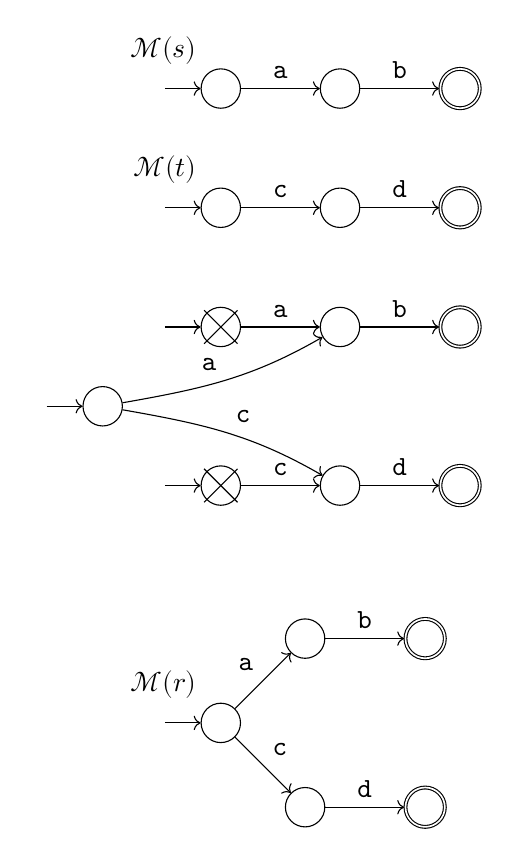
\begin{tikzpicture}
    \tikzset{
      node distance=1cm,
      every state/.append style={minimum size=0.5cm},
      initial text=$ $
    }

    \node[state, initial, label=above left:$\Automaton{\N{s}}$] (x0) {};
    \node[state, right=of x0] (x1) {};
    \node[state, accepting, right=of x1] (x2) {};

    \draw (x0) edge[->] node[auto]{$\Char{a}$} (x1);
    \draw (x1) edge[->] node[auto]{$\Char{b}$} (x2);

    \node[state, initial, label=above left:$\Automaton{\N{t}}$, below=of x0] (y0) {};
    \node[state, right=of y0] (y1) {};
    \node[state, accepting, right=of y1] (y2) {};

    \draw (y0) edge[->] node[auto]{$\Char{c}$} (y1);
    \draw (y1) edge[->] node[auto]{$\Char{d}$} (y2);

    \node[state, initial, below=of y0] (q0) {};
    \path (q0) pic {cross=0.30cm};
    \node[state, right=of q0] (q1) {};
    \node[state, accepting, right=of q1] (q2) {};

    \draw (q0) edge[->] node[auto]{$\Char{a}$} (q1);
    \draw (q1) edge[->] node[auto]{$\Char{b}$} (q2);

    \node[state, initial, below=1.5cm of q0] (p0) {};
    \path (p0) pic {cross=0.30cm};
    \node[state, right=of p0] (p1) {};
    \node[state, accepting, right=of p1] (p2) {};

    \draw (p0) edge[->] node[auto]{$\Char{c}$} (p1);
    \draw (p1) edge[->] node[auto]{$\Char{d}$} (p2);

    \node[state, initial] at ($(q0)!0.5!(p0) - (1.5, 0)$) (n) {};

    \draw (n) edge[->, out=10+0, in=-150+0] node[auto] {$\Char{a}$} (q1);
    \draw (n) edge[->, out=-10+0, in=150+0] node[auto] {$\Char{c}$} (p1);

    \node[state, initial, below=2.5cm of p0, label=above left:$\Automaton{\N{r}}$] (u0) {};
    \node[state, above right=of u0] (u1) {};
    \node[state, accepting, right=of u1] (u2) {};

    \draw (u0) edge[->] node[auto]{$\Char{a}$} (u1);
    \draw (u1) edge[->] node[auto]{$\Char{b}$} (u2);

    \node[state, below right=of u0] (u4) {};
    \node[state, accepting, right=of u4] (u5) {};

    \draw (u0) edge[->] node[auto]{$\Char{c}$} (u4);
    \draw (u4) edge[->] node[auto]{$\Char{d}$} (u5);

  \end{tikzpicture}
\end{center}
\Next

\Special{Poseben primer:} Če nizi v $\Language{s}$ in $\Language{t}$ nimajo skupne predpone bodo znaki na robovih, ki izhajajo iz začetnih stanj $\Automaton{s}$ in $\Automaton{t}$ različni. Nastali končni avtomat bo posledično determinističen.

\Ex

\begin{align*}
  \N{s} &= \Char{a} \Spc \Char{b} \\
  \N{p} &= \Char{a} \Spc \Char{b} \Spc \Char{c} \\
  \N{t} &= \Char{a} \Spc \Char{c} \Spc \Char{d} \\
  \N{r} &= \N{s} \Union \N{p} \Union \N{t} \\
\end{align*}

\begin{center}
  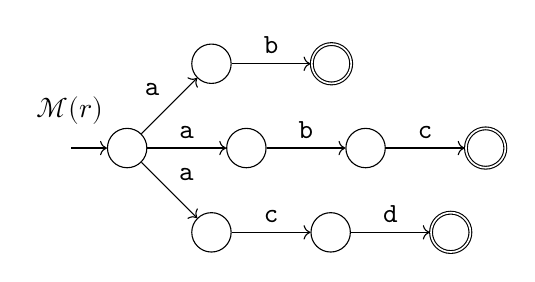
\begin{tikzpicture}
    \tikzset{
      node distance=1cm,
      every state/.append style={minimum size=0.5cm},
      initial text=$ $
    }

    \node[state, initial, label=above left:$\Automaton{\N{r}}$] (u0) {};
    \node[state, right=of u0] (u1) {};
    \node[state, right=of u1] (u2) {};
    \draw (u0) edge[->] node[auto]{$\Char{a}$} (u1);
    \draw (u1) edge[->] node[auto]{$\Char{b}$} (u2);

    \node[state, accepting, right=of u2] (u3) {};
    \draw (u2) edge[->] node[auto]{$\Char{c}$} (u3);

    \node[state, below right=of u0] (u6) {};

    \node[state, right=of u6] (u4) {};
    \node[state, accepting, right=of u4] (u5) {};

    \draw (u0) edge[->] node[auto]{$\Char{a}$} (u6);
    \draw (u6) edge[->] node[auto]{$\Char{c}$} (u4);
    \draw (u4) edge[->] node[auto]{$\Char{d}$} (u5);

    \node[state, above right=of u0] (u7) {};
    \node[state, accepting, right=of u7] (u8) {};

    \draw (u0) edge[->] node[auto]{$\Char{a}$} (u7);
    \draw (u7) edge[->] node[auto]{$\Char{b}$} (u8);

  \end{tikzpicture}
\end{center}

\subsection*{Leva faktorizacija}
Skupno predpono izpostavimo.

\Ex
\begin{align*}
  \N{r} &= \Char{a} \Spc \Char{b} \Union \Char{a} \Spc \Char{b} \Spc \Char{c} \Union \Char{a} \Spc \Char{c} \Spc \Char{d}\\
        &= \Char{a} \Seq (\Char{b} \Union \Char{b} \Spc \Char{c} \Union \Char{c} \Spc \Char{d})\\
        &= \Char{a} \Seq (\Char{b} \Seq (\Null \Union \Char{c}) \Union \Char{c} \Spc \Char{d})
\end{align*}

\begin{center}
  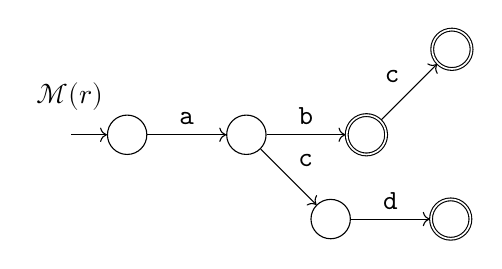
\begin{tikzpicture}
    \tikzset{
      node distance=1cm,
      every state/.append style={minimum size=0.5cm},
      initial text=$ $
    }

    \node[state, initial, label=above left:$\Automaton{\N{r}}$] (u0) {};
    \node[state, right=of u0] (u1) {};
    \node[state, accepting, right=of u1] (u2) {};
    \draw (u0) edge[->] node[auto]{$\Char{a}$} (u1);
    \draw (u1) edge[->] node[auto]{$\Char{b}$} (u2);

    \node[state, accepting, above right=of u2] (u3) {};
    \draw (u2) edge[->] node[auto]{$\Char{c}$} (u3);

    \node[state, below right=of u1] (u4) {};
    \node[state, accepting, right=of u4] (u5) {};

    \draw (u1) edge[->] node[auto]{$\Char{c}$} (u4);
    \draw (u4) edge[->] node[auto]{$\Char{d}$} (u5);

  \end{tikzpicture}
\end{center}


\Special{Poseben primer:} Če sta $s$ in $t$ sestavljena samo z uporabo unije in konkatenacije potem je nastali avtomat unije $\Automaton{r}$ drevo predpon.

\subsection*{Konstrukcija kartezičnega produkta}
Vhod sta $\Automaton{s} = (Q_1, \Alphabet, \delta_1, q_{0,1}, F_1)$ in $\Automaton{t} =(Q_2, \Alphabet, \delta_2, q_{0,2}, F_2)$.

Izhod je nov automat $\Automaton{r} = (Q, \Sigma, \delta, q_{0}, F)$, katerega stanja so kartezični produkt stanj $\Automaton{s}$ in $\Automaton{t}$.

\begin{enumerate}
  \item Začnemo s $q_0 = (q_{0,1}, q_{0,2})$, ki je začetno stanje.
  \item Za vsak znak $\Char{a} \in \Alphabet$, iz trenutnega stanja $q = (q_1, q_2)$ pridobimo nova stanja:
    \begin{equation*}
      q' = (\delta_1(q_1, a), \delta_2(q_2, a))
    \end{equation*}
  \item Za vsako novo stanje dodamo prehod $\delta(q, \Char{a}) = q'$.
  \item Postopek nadaljujemo za vsa tako nastala stanja, ki jih še nismo obravnavali.
  \item Stanje $q = (q_1, q_2)$ je končno, če je $q_1$ ali $q_2$ končno stanje.
\end{enumerate}

Konstrukcija ustvari avtomat, ki se obnaša enako, kot če bi oba vhodna avtomata pognali hkrati.

\Ex

\begin{center}
  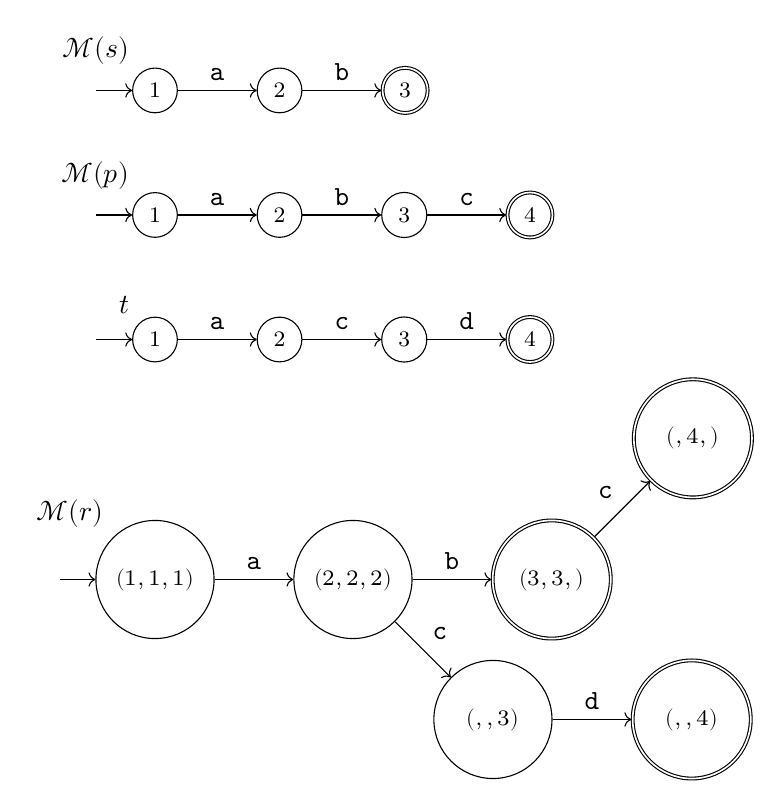
\begin{tikzpicture}
    \tikzset{
      node distance=1cm,
      every state/.append style={minimum size=0.5cm},
      initial text=$ $,
      large/.style={minimum size=1.5cm},
    }

    \node[state, initial, label=above left:$\Automaton{s}$] (x0) {1};
    \node[state, right=of x0] (x1) {2};
    \node[state, accepting, right=of x1] (x2) {3};

    \draw (x0) edge[->] node[auto]{$\Char{a}$} (x1);
    \draw (x1) edge[->] node[auto]{$\Char{b}$} (x2);

    \node[state, initial, label=above left:$\Automaton{p}$, below=of x0] (y0) {1};
    \node[state, right=of y0] (y1) {2};
    \node[state, right=of y1] (y2) {3};
    \node[state, accepting, right=of y2] (y3) {4};

    \draw (y0) edge[->] node[auto]{$\Char{a}$} (y1);
    \draw (y1) edge[->] node[auto]{$\Char{b}$} (y2);
    \draw (y2) edge[->] node[auto]{$\Char{c}$} (y3);

    \node[state, initial, label=above left:$t$, below=of y0] (z0) {1};
    \node[state, right=of z0] (z1) {2};
    \node[state, right=of z1] (z2) {3};
    \node[state, accepting, right=of z2] (z3) {4};

    \draw (z0) edge[->] node[auto]{$\Char{a}$} (z1);
    \draw (z1) edge[->] node[auto]{$\Char{c}$} (z2);
    \draw (z2) edge[->] node[auto]{$\Char{d}$} (z3);

    \node[state, large, initial, below=2cm of z0, label=above left:$\Automaton{r}$] (u0) {$(1,1,1)$};
    \node[state, large, right=of u0] (u1) {$(2, 2, 2)$};
    \node[state, large, accepting, right=of u1] (u2) {$(3,3,\Err)$};
    \draw (u0) edge[->] node[auto]{$\Char{a}$} (u1);
    \draw (u1) edge[->] node[auto]{$\Char{b}$} (u2);

    \node[state, large, accepting, above right=of u2] (u3) {$(\Err, 4, \Err)$};
    \draw (u2) edge[->] node[auto]{$\Char{c}$} (u3);

    \node[state, large, below right=of u1] (u4) {$(\Err,\Err,3)$};
    \node[state, large, accepting, right=of u4] (u5) {$(\Err,\Err,4)$};

    \draw (u1) edge[->] node[auto]{$\Char{c}$} (u4);
    \draw (u4) edge[->] node[auto]{$\Char{d}$} (u5);
  \end{tikzpicture}
\end{center}

Za $(q_1, q_2) \in Q$, če $\acc_1(q_1) \neq \acc_2(q_2)$ potem kot $\acc((q_1, q_2))$ izberemo ali $\acc_1(q_1)$ ali $\acc_2(q_2)$ glede na prioriteto.
Na primer, če združimo avtomata za imena spremenljivk in za ključne besede, vedno izberemo vrednost, ki ustreza avtomatu za ključne besede.
\Next

\subsection*{Primeri}
\subsubsection{Ključne besede}

\begin{align*}
  \N{s} &= \Char{i} \Spc \Char{f} \\
  \N{p} &= \Char{f} \Spc \Char{o} \Spc \Char{r} \\
  \N{t} &= \Char{f} \Spc \Char{o} \Spc \Char{r} \Spc \Char{e} \Spc \Char{a} \Spc \Char{c} \Spc \Char{h} \\
  \N{r} &= \N{s} \Union \N{p} \Union \N{t}
\end{align*}
\Next

\subsection{Opcija}
\Reset

\begin{tcolorbox}[title={Definicija}]
  \begin{equation*}
    \begin{aligned}
      \Opt{s} &= \Null \Union s\\
      \Language{\Opt{s}} &= \{\Str{}\} \cup \Language{s}
    \end{aligned}
  \end{equation*}
\end{tcolorbox}

Ujemanje $s$ 0 ali 1 krat.

Končni avtomat opcije $\Automaton{\Opt{s}}$ lahko sestavimo kot unijo $\Automaton{\Null}$ in $\Automaton{s}$.
Obstaja pa tudi lažji način, $\Automaton{\Opt{s}}$ dobimo tudi, če označimo začetno stanje avtomata $\Automaton{s}$ kot končno.

\begin{center}
  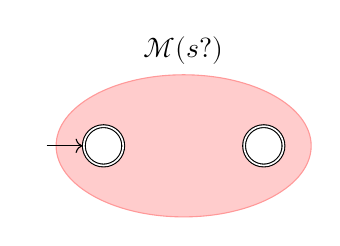
\begin{tikzpicture}
    \tikzset{
      node distance=1cm,
      every state/.append style={fill=white, minimum size=0.5cm},
      initial text=$ $
    }

    %\node[state, initial, accepting] (q0) {};

    \node[state, initial, accepting] (s0) {};
    \node[state, hide, above right=0.15cm and 0.5cm of s0] (s1) {};
    \node[state, hide, below right=0.15cm and 0.5cm of s0] (s2) {};
    \node[state, accepting, right=1.5cm of s0] (sn) {};

    \begin{pgfonlayer}{background}
      \node[fit=(s0) (s1) (s2) (sn), ellip, draw=red!40, fill=red!20, label=above:$\Automaton{\Opt{s}}$] (qm) {};
    \end{pgfonlayer}

  \end{tikzpicture}
\end{center}

\Ex
\begin{center}
  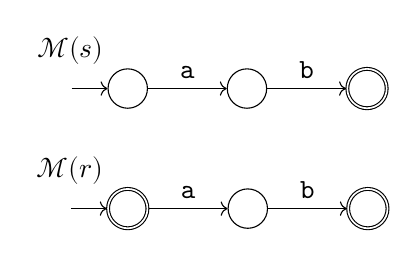
\begin{tikzpicture}
    \tikzset{
      node distance=1cm,
      every state/.append style={minimum size=0.5cm},
      initial text=$ $
    }

    \node[state, initial, label=above left:$\Automaton{\N{s}}$] (x0) {};
    \node[state, right=of x0] (x1) {};
    \node[state, accepting, right=of x1] (x2) {};

    \draw (x0) edge[->] node[auto]{$\Char{a}$} (x1);
    \draw (x1) edge[->] node[auto]{$\Char{b}$} (x2);

    \node[state, initial, accepting, label=above left:$\Automaton{\N{r}}$, below=of x0] (y0) {};
    \node[state, right=of y0] (y1) {};
    \node[state, accepting, right=of y1] (y2) {};

    \draw (y0) edge[->] node[auto]{$\Char{a}$} (y1);
    \draw (y1) edge[->] node[auto]{$\Char{b}$} (y2);
  \end{tikzpicture}
\end{center}

\begin{align*}
  \N{s} &= \Char{a} \Spc \Char{b} \\
  \N{r} &= (\Char{a} \Spc \Char{b})?
\end{align*}

\begin{align*}
  \Language{\N{s}} &= \{\Str{ab}\} \\
  \Language{\N{r}} &= \{\Str{}, \Str{ab}\} \\
\end{align*}

\subsection{Kleene-ovo zaprtje}
\Reset

\begin{tcolorbox}[title={Definicija}]
  \begin{equation*}
    \begin{aligned}
      \Kleene{s} &= \Null \Union s \Union s \Seq s \Union s \Seq s \Seq s \Union \ldots \\
      &= \Rep{s}{0} \Union \Rep{s}{1} \Union \Rep{s}{2} \Union \ldots \\
      &= \Big\vert_{i = 0}^\infty \Rep{s}{i}\\
      \Language{\Kleene{s}} &= \bigcup_{i = 0}^\infty \Language{s^i}
    \end{aligned}
  \end{equation*}
\end{tcolorbox}

Ujemanje $s$ 0 ali več krat.
Z drugimi besedami, $s$ je lahko ponovljen $0, 1, 2, \dots, \infty$ krat.

\begin{tcolorbox}[title={Pravila}]
  \begin{equation*}
    \begin{aligned}
      \Kleene{\Empty} &= \Null\\
      \Kleene{\Null} &= \Null\\
      \Null \Union \Kleene{s} &= \Kleene{s}\\
      \Kleene{s} \Union \Null &= \Kleene{s}\\
      \Kleene{(\Kleene{s})} &= \Kleene{s}\\
      \Kleene{(s \Union t)} &= \Kleene{(\Kleene{s} \Seq t)} \Seq \Kleene{s}\\
      \Kleene{(s \Seq t)} &= \Null \Union s \Seq \Kleene{(t \Seq s)} \Seq t\\
      \Kleene{s} &= (\Null \Union s \Union ... \Union \Rep{s}{i - 1}) \Seq \Kleene{(\Rep{s}{i})}
    \end{aligned}
  \end{equation*}
\end{tcolorbox}

Končni avtomat za Kleeno-ovo zaprtje $\Automaton{\Kleene{s}}$ sestavimo tako:
\begin{enumerate}
  \item Ustvarimo prehod $\delta(q, \Char{a}) = q'$ iz vsakega končnega stanja $q$ v $\Automaton{s}$ v vsako stanje $q'$, ki je direktno dosegljivo iz začetnega stanja istega avtomata.
    Ustvarjen prehod je označen z enakim simbolom $\Char{a}$, kot obstoječi prehod, ki vodi iz začetnega stanja v $q'$.
  \item Začetno stanje označimo kot končno.
\end{enumerate}

\begin{center}
  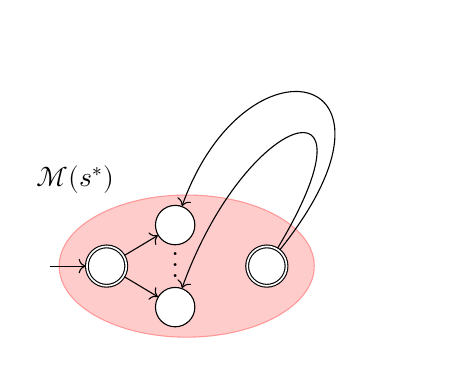
\begin{tikzpicture}
    \tikzset{
      node distance=1cm,
      every state/.append style={fill=white, minimum size=0.5cm},
      initial text=$ $
    }

    \node[state, initial, accepting] (s0) {};
    \node[state, above right=0.15cm and 0.5cm of s0] (s1) {};
    \node[state, below right=0.15cm and 0.5cm of s0] (s2) {};
    \node at ($(s1)!0.5!(s2)$) {\Dots{}};
    \draw (s0) edge[->] (s1);
    \draw (s0) edge[->] (s2);
    \node[state, accepting, right=1.5cm of s0] (sn) {};

    \draw (sn) edge[->, controls={+(2.0,2.5) and +(0.9, 2.5)}] (s1);
    \draw (sn) edge[->, controls={+(1.5,2.5) and +(0.9, 2.5)}] (s2);

    \begin{pgfonlayer}{background}
      \node[fit=(s0) (s1) (s2) (sn), ellip, draw=red!40, fill=red!20, label=above left:$\Automaton{\Kleene{s}}$] (qm) {};
    \end{pgfonlayer}

  \end{tikzpicture}
\end{center}

\Ex
\begin{align*}
  \N{s} &= \Char{a} \\
  \N{r} &= \Kleene{\Char{a}}
\end{align*}

\begin{align*}
  \Language{\N{s}} &= \{\Str{a}\} \\
  \Language{\N{r}} &= \{\Str{}, \Str{a}, \Str{aa}, \Str{aaa}, \dots\} \\
\end{align*}

\begin{center}
  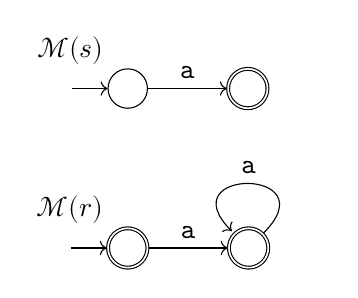
\begin{tikzpicture}
    \tikzset{
      ->,
      node distance=1cm,
      every state/.append style={minimum size=0.5cm},
      initial text=$ $
    }

    \node[state, initial, label=above left:$\Automaton{\N{s}}$] (q0) {};
    \node[state, accepting, right=of q0] (q1) {};

    \draw (q0) edge node[auto]{$\Char{a}$} (q1);

    \node[state, accepting, initial, label=above left:$\Automaton{\N{r}}$, below=1.5cm of q0] (p0) {};
    \node[state, accepting, right=of p0] (p1) {};

    \draw (p0) edge node[auto]{$\Char{a}$} (p1);
    \draw (p1) edge[loop] node[above]{$\Char{a}$} (p1);
  \end{tikzpicture}
\end{center}
\Next

\Ex
\begin{align*}
  \N{s} &= \Char{a} \Spc \Char{b} \\
  \N{r} &= \Kleene{(\Char{a} \Spc \Char{b})}
\end{align*}

\begin{align*}
  \Language{\N{s}} &= \{\Str{ab}\} \\
  \Language{\N{r}} &= \{\Str{}, \Str{ab}, \Str{abab}, \Str{ababab}, \dots\}
\end{align*}

\begin{center}
  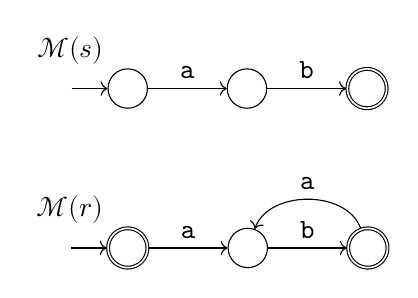
\begin{tikzpicture}
    \tikzset{
      ->,
      node distance=1cm,
      every state/.append style={minimum size=0.5cm},
      initial text=$ $
    }

    \node[state, initial, label=above left:$\Automaton{\N{s}}$] (q0) {};
    \node[state, right=of q0] (q1) {};
    \node[state, accepting, right=of q1] (q2) {};

    \draw (q0) edge node[auto]{$\Char{a}$} (q1);
    \draw (q1) edge node[auto]{$\Char{b}$} (q2);

    \node[state, accepting, label=above left:$\Automaton{\N{r}}$, initial, below=1.5cm of q0] (p0) {};
    \node[state, right=of p0] (p1) {};
    \node[state, accepting, right=of p1] (p2) {};

    \draw (p0) edge node[auto]{$\Char{a}$} (p1);
    \draw (p1) edge node[auto]{$\Char{b}$} (p2);
    \draw (p2) edge[bend right=70] node[above]{$\Char{a}$} (p1);
  \end{tikzpicture}
\end{center}
\Next

\Ex

\begin{align*}
  \N{s} &= \Char{c}\\
  \N{t} &= \Kleene{(\Char{a} \Spc \Char{b})}\\
  \N{r} &= \Char{c} \Seq \Kleene{(\Char{a} \Spc \Char{b})}
\end{align*}

\begin{align*}
  \Language{\N{s}} &= \{\Str{c}\} \\
  \Language{\N{t}} &= \{\Str{}, \Str{ab}, \Str{abab}, \Str{ababab}, \dots\}\\
  \Language{\N{r}} &= \{\Str{c}, \Str{cab}, \Str{cabab}, \Str{cababab}, \dots\}
\end{align*}

\begin{center}
  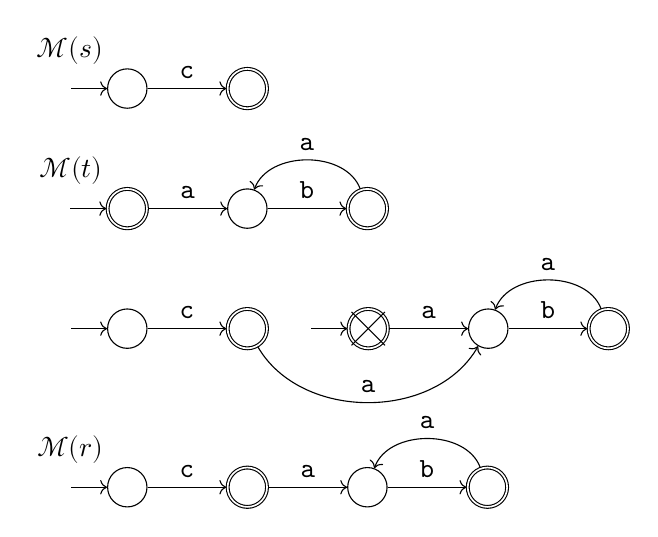
\begin{tikzpicture}
    \tikzset{
      node distance=1cm,
      every state/.append style={minimum size=0.5cm},
      initial text=$ $
    }

    \node[state, initial, label=above left:$\Automaton{\N{s}}$] (x0) {};
    \node[state, accepting, right=of x0] (x1) {};

    \draw (x0) edge[->] node[auto]{$\Char{c}$} (x1);

    \node[state, initial, accepting, label=above left:$\Automaton{\N{t}}$, below=of x0] (y0) {};
    \node[state, right=of y0] (y1) {};
    \node[state, accepting, right=of y1] (y2) {};

    \draw (y0) edge[->] node[auto]{$\Char{a}$} (y1);
    \draw (y1) edge[->] node[auto]{$\Char{b}$} (y2);
    \draw (y2) edge[bend right=70, ->] node[above]{$\Char{a}$} (y1);

    \node[state, initial, below=of y0] (q0) {};
    \node[state, accepting, right=of q0] (q1) {};

    \draw (q0) edge[->] node[auto]{$\Char{c}$} (q1);

    \node[state, initial, accepting, right=of q1] (p0) {};
    \path (p0) pic {cross=0.30cm};
    \node[state, right=of p0] (p1) {};
    \node[state, accepting, right=of p1] (p2) {};

    \draw (p0) edge[->] node[auto]{$\Char{a}$} (p1);
    \draw (p1) edge[->] node[auto]{$\Char{b}$} (p2);

    \draw (q1) edge[->, bend right=60] node[auto]{$\Char{a}$} (p1);
    \draw (p2) edge[bend right=70, ->] node[above]{$\Char{a}$} (p1);

    \node[state, initial, label=above left:$\Automaton{\N{r}}$, below=1.5cm of q0] (s0) {};
    \node[state, accepting, right=of s0] (s1) {};
    \node[state, right=of s1] (s3) {};
    \node[state, accepting, right=of s3] (s4) {};

    \draw (s0) edge[->] node[auto]{$\Char{c}$} (s1);
    \draw (s1) edge[->] node[auto]{$\Char{a}$} (s3);
    \draw (s3) edge[->] node[auto]{$\Char{b}$} (s4);
    \draw (s4) edge[bend right=70, ->] node[above]{$\Char{a}$} (s3);
  \end{tikzpicture}
\end{center}
\Next

\Ex
\begin{align*}
  \N{s} &= \Char{a} \Union \Char{b}\\
  \N{r} &= \Kleene{(\Char{a} \Union \Char{b})}
\end{align*}

\begin{align*}
  \Language{\N{s}} &= \{\Str{a}, \Str{b}\} \\
  \Language{\N{r}} &= \{\Null, \Str{a}, \Str{b}, \Str{aa}, \Str{ab}, \Str{ba}, \Str{bb}, \dots\}\\
\end{align*}

\begin{center}
  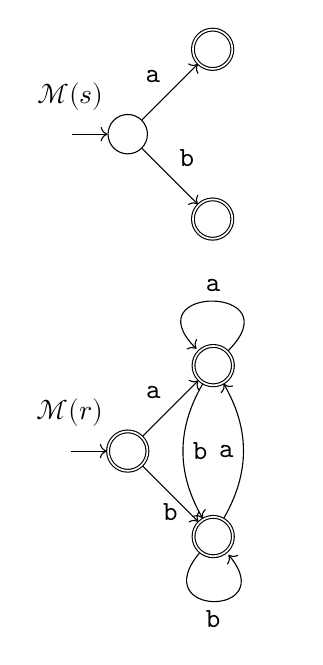
\begin{tikzpicture}
    \tikzset{
      ->,
      node distance=1cm,
      every state/.append style={minimum size=0.5cm},
      initial text=$ $
    }

    \node[state, initial, label=above left:$\Automaton{\N{s}}$] (q0) {};
    \node[state, accepting, above right=of q0] (q1) {};
    \node[state, accepting, below right=of q0] (q2) {};

    \draw (q0) edge node[auto]{$\Char{a}$} (q1);
    \draw (q0) edge node[auto]{$\Char{b}$} (q2);

    \node[state, accepting, label=above left:$\Automaton{\N{r}}$, initial, below=3.5cm of q0] (p0) {};
    \node[state, accepting, above right=of p0] (p1) {};
    \node[state, accepting, below right=of p0] (p2) {};

    \draw (p0) edge node[auto]{$\Char{a}$} (p1);
    \draw (p0) edge node[below]{$\Char{b}$} (p2);
    \draw (p1) edge[bend right] node[auto]{$\Char{b}$} (p2);
    \draw (p2) edge[bend right] node[auto]{$\Char{a}$} (p1);
    \draw (p1) edge[loop] node[above]{$\Char{a}$} (p1);
    \draw (p2) edge[in=-50,out=-130, loop] node[below]{$\Char{b}$} (p2);
  \end{tikzpicture}
\end{center}
\Next

\Ex
\begin{equation*}
\begin{aligned}
  \N{r} &= \Char{a} \Spc \Char{b} \Union \Kleene{\Char{a}}\\
  &= \Char{a} \Spc \Char{b} \Union \Null \Union \Char{a} \Union \Char{a} \Spc \Char{a} \Union \Char{a} \Spc \Char{a} \Spc \Char{a} \Union \dots\\
  &=  \Null \Union \Char{a} \Spc \Char{b} \Union \Char{a} \Union \Char{a} \Spc \Char{a} \Union \Char{a} \Spc \Char{a} \Spc \Char{a} \Union \dots\\
  &= \Null \Union \Char{a} \Seq (\Char{b} \Union \Null \Union \Char{a} \Union \Char{a} \Spc \Char{a} \Union \dots)\\
  &= \Null \Union \Char{a} \Seq (\Char{b} \Union \Kleene{\Char{a}})\\
  &= \Opt{(\Char{a} \Seq (\Char{b} \Union \Kleene{\Char{a}}))}\\
\end{aligned}
\end{equation*}

\begin{center}
  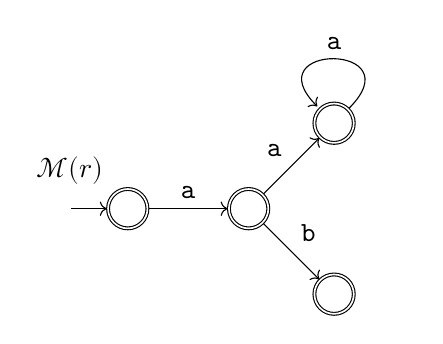
\begin{tikzpicture}
    \tikzset{
      ->,
      node distance=1cm,
      every state/.append style={minimum size=0.5cm},
      initial text=$ $
    }

    \node[state, initial, accepting, label=above left:$\Automaton{\N{r}}$] (i) {};

    \node[state, accepting, right=of i] (q0) {};
    \node[state, accepting, above right=of q0] (q1) {};
    \node[state, accepting, below right=of q0] (q2) {};

    \draw (i) edge node[auto]{$\Char{a}$} (q0);
    \draw (q0) edge node[auto]{$\Char{a}$} (q1);
    \draw (q0) edge node[auto]{$\Char{b}$} (q2);
    \draw (q1) edge[loop] node[above]{$\Char{a}$} (q2);
  \end{tikzpicture}
\end{center}


\subsection{Pozitivno zaprtje}
\Reset

\begin{tcolorbox}[title={Definicija}]
  \begin{equation*}
    \begin{aligned}
      \KleenePlus{s} &= s \Union s \Seq s \Union s \Seq s \Seq s \Union \ldots \\
      &= \Rep{s}{1} \Union \Rep{s}{2} \Union \ldots \\
      &= \Big\vert_{i = 1}^\infty \Rep{s}{i}\\
      \Language{\KleenePlus{s}} &= \bigcup_{i = 1}^\infty \Language{s^i}\\[1em]
      \Kleene{s} &= \Null \Union \KleenePlus{s} = \Opt{(\KleenePlus{s})} = \KleenePlus{(\Opt{s})}\\
      \Language{\Kleene{r}} &= \{\Str{}\} \cup \Language{\KleenePlus{r}}
    \end{aligned}
  \end{equation*}
\end{tcolorbox}

Ujemanje $s$ 1 ali več krat.
Z drugimi besedami, $s$ je lahko ponovljen $1, 2, \dots, \infty$ krat.

Končen avtomat pozitivnega zaprtja sestavimo enako, kot za Kleene-ovo zaprtje, z razliko, da pustimo začetno stanje brez sprememb.
\begin{center}
  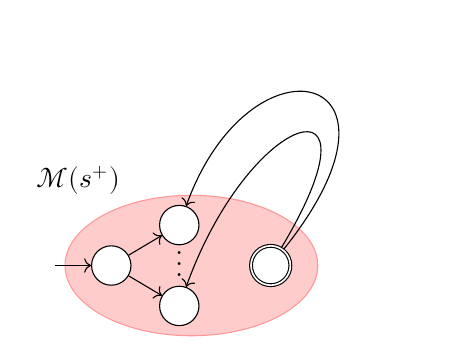
\begin{tikzpicture}
    \tikzset{
      node distance=1cm,
      every state/.append style={fill=white, minimum size=0.5cm},
      initial text=$ $
    }

    \node[state, initial] (s0) {};
    \node[state, above right=0.15cm and 0.5cm of s0] (s1) {};
    \node[state, below right=0.15cm and 0.5cm of s0] (s2) {};
    \node at ($(s1)!0.5!(s2)$) {\Dots{}};
    \draw (s0) edge[->] (s1);
    \draw (s0) edge[->] (s2);
    \node[state, accepting, right=1.5cm of s0] (sn) {};

    \draw (sn) edge[->, controls={+(2.0,2.5) and +(0.9, 2.5)}] (s1);
    \draw (sn) edge[->, controls={+(1.5,2.5) and +(0.9, 2.5)}] (s2);

    \begin{pgfonlayer}{background}
      \node[fit=(s0) (s1) (s2) (sn), ellip, draw=red!40, fill=red!20, label=above left:$\Automaton{\KleenePlus{s}}$] (qm) {};
    \end{pgfonlayer}

  \end{tikzpicture}
\end{center}

\Ex
\begin{align*}
  \N{s} &= \Char{a} \\
  \N{r} &= \KleenePlus{\Char{a}}
\end{align*}

\begin{align*}
  \Language{\N{s}} &= \{\Str{a}\} \\
  \Language{\N{r}} &= \{\Str{a}, \Str{aa}, \Str{aaa}, \dots\} \\
\end{align*}

\begin{center}
  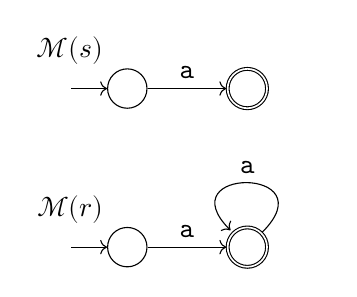
\begin{tikzpicture}
    \tikzset{
      ->,
      node distance=1cm,
      every state/.append style={minimum size=0.5cm},
      initial text=$ $
    }

    \node[state, initial, label=above left:$\Automaton{\N{s}}$] (q0) {};
    \node[state, accepting, right=of q0] (q1) {};

    \draw (q0) edge node[auto]{$\Char{a}$} (q1);

    \node[state, initial, label=above left:$\Automaton{\N{r}}$, below=1.5cm of q0] (p0) {};
    \node[state, accepting, right=of p0] (p1) {};

    \draw (p0) edge node[auto]{$\Char{a}$} (p1);
    \draw (p1) edge[loop] node[above]{$\Char{a}$} (p1);
  \end{tikzpicture}
\end{center}
\Next

\Ex
\begin{align*}
  \N{s} &= \Char{a}? \\
  \N{r} &= \KleenePlus{(\Char{a}?)}
\end{align*}

\begin{align*}
  \Language{\N{s}} &= \{\Str{}, \Str{a}\} \\
  \Language{\N{r}} &= \{\Str{}, \Str{a}, \Str{aa}, \Str{aaa}, \dots\} \\
\end{align*}

\begin{center}
  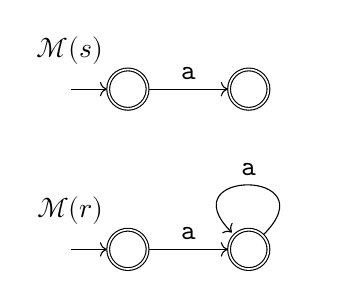
\begin{tikzpicture}
    \tikzset{
      ->,
      node distance=1cm,
      every state/.append style={minimum size=0.5cm},
      initial text=$ $
    }

    \node[state, accepting, initial, label=above left:$\Automaton{\N{s}}$] (q0) {};
    \node[state, accepting, right=of q0] (q1) {};

    \draw (q0) edge node[auto]{$\Char{a}$} (q1);

    \node[state, accepting, initial, label=above left:$\Automaton{\N{r}}$, below=1.5cm of q0] (p0) {};
    \node[state, accepting, right=of p0] (p1) {};

    \draw (p0) edge node[auto]{$\Char{a}$} (p1);
    \draw (p1) edge[loop] node[above]{$\Char{a}$} (p1);
  \end{tikzpicture}
\end{center}
\Next

\subsection*{Primeri}
\subsubsection{Števila}
\begin{align*}
  \N{s} &= \{\Char{0}, \dots, \Char{9}\} \\
  \N{r} &= \KleenePlus{\N{s}}
\end{align*}
\Next

\subsubsection{Naravna števila}
\begin{equation*}
  \Language{\N{r}} = \{\Str{1}, \Str{2}, \dots\}
\end{equation*}
\Next

\subsubsection{Cela števila}
\begin{align*}
  \N{s} &= \{\Char{0}, \dots, \Char{9}\} \\
  \N{r} &= (\Char{+} \Union \Char{-}) \Seq \KleenePlus{\N{s}}
\end{align*}
\Next

\subsubsection{Heksadecimalna števila}
\begin{equation*}
  \Language{\N{r}} = \{\Str{0x0}, \Str{0x1}, \dots, \Str{0xA}, \dots, \Str{0xFFFF}, \dots\}
\end{equation*}
\Next

\subsubsection{Barve}
\begin{equation*}
  \Language{\N{r}} = \{\Str{\#000000}, \dots, \Str{\#FFFFFF}\}
\end{equation*}
\Next

\subsubsection{Števila s plavajočo vejico}
\begin{align*}
  \N{s} &= \{\Char{0}, \dots, \Char{9}\} \\
  \N{r} &= (\Char{+} \Union \Char{-}) \Seq \KleenePlus{\N{s}} \Spc \Char{.} \Spc \Kleene{\N{s}}
\end{align*}
\Next

\subsubsection{Imena spremenljivk}
\begin{align*}
  \N{l} &= \{\Char{a}, \dots, \Char{z}\} \\
  \N{r} &= \KleenePlus{\N{l}}
\end{align*}

\begin{center}
  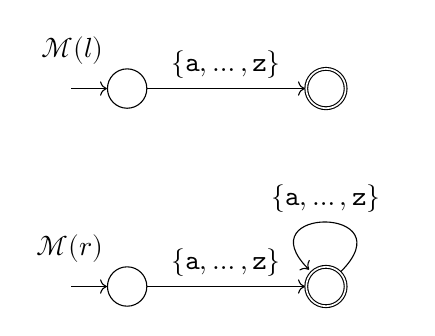
\begin{tikzpicture}
    \tikzset{
      ->,
      node distance=1cm,
      every state/.append style={minimum size=0.5cm},
      initial text=$ $
    }

    \node[state, initial, label=above left:$\Automaton{\N{l}}$] (q0) {};
    \node[state, accepting, right=2cm of q0] (q1) {};

    \draw (q0) edge node[auto]{$\{\Char{a}, \dots, \Char{z}\}$} (q1);

    \node[state, initial, label=above left:$\Automaton{\N{r}}$, below=2.0cm of q0] (p0) {};
    \node[state, accepting, right=2cm of p0] (p1) {};

    \draw (p0) edge node[auto]{$\{\Char{a}, \dots, \Char{z}\}$} (p1);
    \draw (p1) edge[loop] node[above]{$\{\Char{a}, \dots, \Char{z}\}$} (p1);
  \end{tikzpicture}
\end{center}
\Next

\subsubsection{Ključne besede in imena spremenljivk}
\begin{align*}
  \N{i} &= \KleenePlus{\{\Char{a}, \dots, \Char{z}\}}\\
  \N{k} &= \Char{a} \Spc \Char{b} \Union \Char{a} \Spc \Char{b} \Spc \Char{c} \Union \Char{a} \Spc \Char{c} \Spc \Char{d}\\
  \N{r} &= \N{i} \Union \N{k}
\end{align*}

\begin{equation*}
  A = \{\Char{a}, \dots, \Char{z}\}
\end{equation*}

Gre tudi z izpostavljanjem, vendar je nastali regularni izraz precej kompleksen.
\begin{equation*}
\begin{aligned}
  \N{r} &= \Char{a} \Spc \Char{b} \Union \Char{a} \Spc \Char{b} \Spc \Char{c} \Union \Char{a} \Spc \Char{c} \Spc \Char{d} \Union \KleenePlus{A}\\
  &= \underline{\Char{a}} \Seq (\Char{b} \Union \Char{b} \Spc \Char{c} \Union \Char{c} \Spc \Char{d} \Union \Kleene{A}) \Union (A - \{\Char{a}\}) \Seq \Kleene{A}\\ 
  &= \Char{a} \Seq (\Null \Union \underline{\Char{b}} \Seq (\not\Null \Union \Char{c} \Union \Kleene{A}) \Union \underline{\Char{c}} \Seq (\Char{d} \Union \Kleene{A}) \Union (A - \{\Char{b}, \Char{c}\}) \Seq \Kleene{A}) \Union (A - \{\Char{a}\}) \Seq \Kleene{A} \\
  &= \Char{a} \Seq (\Null \Union \Char{b} \Seq (\Char{c} \Union \Kleene{A}) \Union \Char{c} \Seq (\Char{d} \Union \Kleene{A}) \Union (A - \{\Char{b}, \Char{c}\}) \Seq \Kleene{A}) \Union (A - \{\Char{a}\}) \Seq \Kleene{A}\\
  &= \Char{a} \Seq (\Null \Union \Char{b} \Seq (\Null \Union \underline{\Char{c}} \Seq (\not\Null \Union \Kleene{A}) \Union (A - \{\Char{c}\}) \Seq \Kleene{A}) \Union \Char{c} \Seq (\Char{d} \Union \Kleene{A}) \Union (A - \{\Char{b}, \Char{c}\}) \Seq \Kleene{A}) \Union (A - \{\Char{a}\}) \Seq \Kleene{A}\\
  &= \Char{a} \Seq (\Null \Union \Char{b} \Seq (\Null \Union \Char{c} \Seq \Kleene{A} \Union (A - \{\Char{c}\}) \Seq \Kleene{A}) \Union \Char{c} \Seq (\Char{d} \Union \Kleene{A}) \Union (A - \{\Char{b}, \Char{c}\}) \Seq \Kleene{A}) \Union (A - \{\Char{a}\}) \Seq \Kleene{A}\\
  &= \Char{a} \Seq (\Null \Union \Char{b} \Seq (\Null \Union \Char{c} \Seq \Kleene{A} \Union (A - \{\Char{c}\}) \Seq \Kleene{A}) \Union \Char{c} \Seq (\Null \Union \underline{\Char{d}} \Seq (\not\Null \Union \Kleene{A}) \Union (A - \{\Char{d}\}) \Seq \Kleene{A}) \Union (A - \{\Char{b}, \Char{c}\}) \Seq \Kleene{A}) \Union (A - \{\Char{a}\}) \Seq \Kleene{A}\\
  &= \Char{a} \Seq (\Null \Union \Char{b} \Seq (\Null \Union \Char{c} \Seq \Kleene{A} \Union (A - \{\Char{c}\}) \Seq \Kleene{A}) \Union \Char{c} \Seq (\Null \Union \Char{d} \Seq \Kleene{A} \Union (A - \{\Char{d}\}) \Seq \Kleene{A}) \Union (A - \{\Char{b}, \Char{c}\}) \Seq \Kleene{A}) \Union (A - \{\Char{a}\}) \Seq \Kleene{A}\\
\end{aligned}
\end{equation*}

Zato raje uporabimo konstrukcijo kartezičnega produkta.
\begin{align*}
  \acc_{\N{i}}(2) &= 1 \\[1em]
  \acc_{\N{k}}(3) &= 2 \\
  \acc_{\N{k}}(4) &= 2 \\
  \acc_{\N{k}}(6) &= 2 \\
\end{align*}

\begin{center}
  \begin{tikzpicture}
    \tikzset{
      ->,
      node distance=1cm,
      every state/.append style={minimum size=0.5cm},
      initial text=$ $
    }

    \node[state, initial, label=above left:$\Automaton{\N{i}}$, below=2.0cm of q0] (p0) {1};
    \node[state, accepting, right=2cm of p0] (p1) {2};

    \draw (p0) edge node[auto]{$\{\Char{a}, \dots, \Char{z}\}$} (p1);
    \draw (p1) edge[loop] node[above]{$\{\Char{a}, \dots, \Char{z}\}$} (p1);

    \node[state, initial, label=above left:$\Automaton{\N{k}}$, below=1.5cm of p0] (u0) {1};
    \node[state, right=of u0] (u1) {2};
    \node[state, accepting, right=of u1] (u2) {3};
    \draw (u0) edge[->] node[auto]{$\Char{a}$} (u1);
    \draw (u1) edge[->] node[auto]{$\Char{b}$} (u2);

    \node[state, accepting, right=of u2] (u3) {4};
    \draw (u2) edge[->] node[auto]{$\Char{c}$} (u3);

    \node[state, below right=of u1] (u4) {5};
    \node[state, accepting, right=of u4] (u5) {6};

    \draw (u1) edge[->] node[auto]{$\Char{c}$} (u4);
    \draw (u4) edge[->] node[auto]{$\Char{d}$} (u5);
  \end{tikzpicture}
\end{center}

\begin{center}
  \begin{tikzpicture}
    \tikzset{
      ->,
      node distance=1cm,
      every state/.append style={minimum size=0.5cm},
      large/.style={minimum size=1.2cm},
      initial text=$ $
    }

    \node[state, large, initial, label=above left:$\Automaton{\N{r}}$] (v0) {$(1,1)$};
    \node[state, large, accepting, right=of v0] (v1) {(2,2)};
    \node[state, large, accepting, right=of v1] (v2) {$(2, 3)$};
    \draw (v0) edge[->] node[auto]{$\Char{a}$} (v1);
    \draw (v1) edge[->] node[auto]{$\Char{b}$} (v2);

    \node[state, large, accepting, right=of v2] (v3) {$(2, 4)$};
    \draw (v2) edge[->] node[auto]{$\Char{c}$} (v3);

    \node[state, large, accepting, below right=of v1] (v4) {$(2, 5)$};
    \node[state, large, accepting, right=of v4] (v5) {$(2, 6)$};

    \draw (v1) edge[->] node[auto]{$\Char{c}$} (v4);
    \draw (v4) edge[->] node[auto]{$\Char{d}$} (v5);

    \node[state, large, accepting, above=2cm of v1] (s) {$(2, \Err)$};
    \draw (v0) edge[->, bend left] node[auto]{$A - \{\Char{a}\}$} (s);
    \draw (v1) edge[->, bend right] node[auto]{$A - \{\Char{b}, \Char{c}\}$} (s);
    \draw (v2) edge[->, bend right] node[right]{$A - \{\Char{c}\}$} (s);
    \draw (v3) edge[->, bend right=50] node[above right]{$A$} (s);
    \draw (v4) edge[->, out=-150, in=170, looseness=3] node[left ]{$A - \{\Char{d}\}$} (s);
    \draw (v5) edge[->, out=0, in=45, looseness=2] node[right]{$A$} (s);
    \draw (s) edge[->, loop] node[above]{$A$} (s);
  \end{tikzpicture}
\end{center}
\begin{align*}
  \acc_{\N{r}}((2, \Err)) &= 1 \\
  \acc_{\N{r}}((2, 2)) &= 1 \\
  \acc_{\N{r}}((2, 3)) &= 2 \\
  \acc_{\N{r}}((2, 4)) &= 2 \\
  \acc_{\N{r}}((2, 5)) &= 1 \\
  \acc_{\N{r}}((2, 6)) &= 2 \\
\end{align*}

\Special{Poseben primer:} Potrebno je samo eno dodatno stanje $(2, \Err)$, v primerjavi z avtomatom za ključne besede.
Stanje $(2, \Err)$ deluje kot ponor.
Množice znakov $A - D$ lahko implementiramo tako, da najprej naredimo vse prehode za A in jih potem "povozimo" s prehodi za D.
\Next

\chapter{Gramatike}

\begin{tcolorbox}[title={Definicija}]
  \begin{equation*}
    \begin{aligned}
      G = (\Terminals, \NonTerminals, \Productions, \NT{S})
    \end{aligned}
  \end{equation*}
\end{tcolorbox}

\section{Osnovne gramatike} 
Gramatike so v veliki meri sestavljene iz naslednjih osnovnih vzorcev.

\subsubsection{Seznam}
\begin{equation*}
  \begin{aligned}[t]
    \NT{L} &\Arrow \T{i} \Spc \NT{L} \Union \Null\\[1em]
    \NT{Numbers} &\Arrow \T{num} \Spc \NT{Numbers} \Union \Null\\[1em]
    \T{num} &= \KleenePlus{\{\Char{0}, \dots, \Char{9}\}}
  \end{aligned}
\end{equation*}
\begin{lstlisting}
$\Null$
1
1 2
1 2 3
\end{lstlisting}

\subsubsection{Seznam z ločilom}
\begin{equation*}
  \begin{aligned}[t]
    \NT{L} &\Arrow \T{i} \Spc \T{s} \Spc \NT{L} \Union \Null\\[1em]
    \NT{Numbers} &\Arrow \T{num} \Spc \T{sep} \Spc \NT{Numbers} \Union \Null\\[1em]
    \T{num} &= \KleenePlus{\{\Char{0}, \dots, \Char{9}\}}\\
    \T{sep} &= \Char{;}
  \end{aligned}
\end{equation*}
\begin{lstlisting}
$\Null$
1;
1; 2;
1; 2; 3;
\end{lstlisting}
Ločilo je tudi na koncu.

\subsubsection{Neprazen seznam}
Da lahko neprazen seznam razpoznamo z LL(1) razpoznavalnikom moramo gramatiko preoblikovati.
\begin{equation*}
  \begin{aligned}[t]
    \NT{L} &\Arrow \T{i} \Spc \NT{L} \Union \T{i}\\[1em]
    \NT{L} &\Arrow \T{i} \Seq (\NT{L} \Union \Null)\text{\quad izpostavimo \T{i}}\\[1em]
    \NT{L} &\Arrow \T{i} \Spc \NT{L'}\\
    \NT{L'} &\Arrow \NT{L} \Union \Null \text{\quad oklepaje spremenimo v novo produkcijo}\\[1em]
    \NT{L} &\Arrow \T{i} \Spc \NT{L'}\\
    \NT{L'} &\Arrow \T{i} \Spc \NT{L'} \Union \Null \text{\quad zamenjamo \NT{L} z desno stranjo}\\[1em]
    \NT{L} &\Arrow \T{i} \Seq \Kleene{\T{i}}\\[1em]
    \NT{Numbers} &\Arrow \T{num} \Spc \NT{Numbers} \Union \T{num}\\[1em]
    \NT{Numbers} &\Arrow \T{num} \Spc \NT{Numbers'}\\
    \NT{Numbers'} &\Arrow \T{num} \Spc \NT{Numbers'} \Union \Null\\[1em]
    \NT{Numbers} &\Arrow \T{num} \Spc \Kleene{\T{num}}\\[1em]
    \T{num} &= \KleenePlus{\{\Char{0}, \dots, \Char{9}\}}
  \end{aligned}
\end{equation*}
\begin{lstlisting}
1
1 2
1 2 3
\end{lstlisting}

\subsubsection{Neprazen seznam z ločilom}
\begin{equation*}
  \begin{aligned}[t]
    \NT{L} &\Arrow \T{i} \Spc \T{s} \Spc \NT{L} \Union \T{i}\\[1em]
    \NT{L} &\Arrow \T{i} \Seq (\T{s} \Spc \NT{L} \Union \Null)\text{\quad izpostavimo \T{i}}\\[1em]
    \NT{L} &\Arrow \T{i} \Spc \NT{L'}\\
    \NT{L'} &\Arrow \T{s} \Spc \NT{L} \Union \Null \text{\quad oklepaje spremenimo v novo produkcijo}\\[1em]
    \NT{L} &\Arrow \T{i} \Spc \NT{L'}\\
    \NT{L'} &\Arrow \T{s} \Spc \T{i} \Spc \NT{L'} \Union \Null \text{\quad zamenjamo \NT{L} z desno stranjo}\\[1em]
    \NT{L} &\Arrow \T{i} \Seq \Kleene{(\T{s} \Spc \T{i})}\\[1em]
    \NT{Numbers} &\Arrow \T{num} \Spc \T{sep} \Spc \NT{Numbers} \Union \T{num}\\[1em]
    \NT{Numbers} &\Arrow \T{num} \Spc \NT{Numbers'}\\
    \NT{Numbers'} &\Arrow \T{sep} \Spc \T{num} \Spc \NT{Numbers'} \Union \Null\\[1em]
    \NT{Numbers} &\Arrow \T{num} \Spc \Kleene{(\T{sep} \Spc \T{num})}\\[1em]
    \T{num} &= \KleenePlus{\{\Char{0}, \dots, \Char{9}\}}\\
    \T{sep} &= \Char{+}
  \end{aligned}
\end{equation*}
\begin{lstlisting}
1
1 + 2
1 + 2 + 3
\end{lstlisting}
Ločila ni na koncu.

\subsubsection{Opcijsko}
\begin{equation*}
  \begin{aligned}[t]
    \NT{B} &\Arrow \NT{I} \Spc \T{i}\\
    \NT{I} &\Arrow \T{i} \Union \Null \\[1em]
    \NT{Val} &\Arrow \NT{Sign} \Spc \T{num}\\
    \NT{Sign} &\Arrow \T{plus} \Union \T{minus} \Union \Null\\[1em]
    \T{num} &= \KleenePlus{\{\Char{0}, \dots, \Char{9}\}}\\
    \T{plus} &= \Char{+}\\
    \T{minus} &= \Char{-}
  \end{aligned}
\end{equation*}
\begin{lstlisting}
1
+1
-1
\end{lstlisting}

\subsubsection{Vsebovanje}
Nekaj znotraj nečesa.
\begin{equation*}
  \begin{aligned}[t]
    \NT{B} &\Arrow \T{l} \Spc \T{I} \Spc \T{r}\\
    \NT{I} &\Arrow \T{i}\\[1em]
    \NT{Box} &\Arrow \T{lbrak} \Spc \NT{Val} \Spc \T{rbrak}\\
    \NT{Val} &\Arrow \T{num} \Union \T{star}\\[1em]
    \T{num} &= \KleenePlus{\{\Char{0}, \dots, \Char{9}\}}\\
    \T{lbrak} &= \Char{[}\\
    \T{rbrak} &= \Char{]}\\
    \T{star} &= \Char{*}
  \end{aligned}
\end{equation*}
\begin{lstlisting}
[*]
[1]
\end{lstlisting}

\begin{equation*}
  \begin{aligned}[t]
    \NT{B} &\Arrow \T{l} \Spc \T{L} \Spc \T{r}\\
    \NT{L} &\Arrow \T{i} \Spc \NT{L'}\\
    \NT{L'} &\Arrow \T{s} \Spc \T{i} \Spc \NT{L'} \Union \Null\\[1em]
    \NT{Box} &\Arrow \T{lbrak} \Spc \NT{Numbers} \Spc \T{rbrak}\\
    \NT{Numbers} &\Arrow \T{num} \Spc \NT{Numbers'}\\
    \NT{Numbers'} &\Arrow \T{sep} \Spc \T{num} \Spc \NT{Numbers'} \Union \Null\\[1em]
    \T{num} &= \KleenePlus{\{\Char{0}, \dots, \Char{9}\}}\\
    \T{lbrak} &= \Char{[}\\
    \T{rbrak} &= \Char{]}\\
    \T{sep} &= \Char{+}
  \end{aligned}
\end{equation*}
\begin{lstlisting}
[1]
[1 + 2]
[1 + 2 + 3]
\end{lstlisting}

\subsubsection{Gnezdenje}

\begin{equation*}
  \begin{aligned}[t]
    \NT{B} &\Arrow \T{l} \Spc \NT{B} \Spc \T{r} \Union \NT{I}\\[1em]
    \NT{I} &\Arrow \T{i}\\
    \NT{Box} &\Arrow \T{lbrak} \Spc \NT{Box} \Spc \T{rbrak} \Union \NT{Val}\\
    \NT{Val} &\Arrow \T{num} \Union \T{star}\\[1em]
    \T{num} &= \KleenePlus{\{\Char{0}, \dots, \Char{9}\}}\\
    \T{lbrak} &= \Char{[}\\
    \T{rbrak} &= \Char{]}\\
    \T{star} &= \Char{*}
  \end{aligned}
\end{equation*}
\begin{lstlisting}
[*]
[[[1]]]
[[[[[[[1]]]]]]]
\end{lstlisting}

\begin{equation*}
  \begin{aligned}[t]
    \NT{L} &\Arrow \NT{I} \Spc \NT{L'}\\
    \NT{L'} &\Arrow \T{s} \Spc \NT{I} \Spc \NT{L'} \Union \Null\\
    \NT{I} &\Arrow \T{i} \Union \NT{L}\\[1em]
    \NT{Numbers} &\Arrow \T{Val} \Spc \NT{Numbers'}\\
    \NT{Numbers'} &\Arrow \T{sep} \Spc \T{Val} \Spc \NT{Numbers'} \Union \Null\\
    \NT{Val} &\Arrow \T{num} \Union \T{lbrak} \Spc \NT{Numbers} \Spc \T{rbrak}\\[1em]
    \T{num} &= \KleenePlus{\{\Char{0}, \dots, \Char{9}\}}\\
    \T{lbrak} &= \Char{[}\\
    \T{rbrak} &= \Char{]}\\
    \T{sep} &= \Char{+}
  \end{aligned}
\end{equation*}
\begin{lstlisting}
[1]
[[[1] + [2] + [3]]]
[[1 + [2] + [1 + 2 + 3]]]
\end{lstlisting}

\subsection*{Izrazi}

"Naravna" gramatika za izraze.
\begin{align*}
  \NT{Start} &\Arrow \NT{Expr}\\
  \NT{Expr} &\Arrow \NT{Expr} \Spc \T{plus} \Spc \NT{Expr}\\
            &\Union \NT{Expr} \Spc \T{minus} \Spc \NT{Expr}\\
            &\Union \NT{Expr} \Spc \T{times} \Spc \NT{Expr}\\
            &\Union \NT{Expr} \Spc \T{divide} \Spc \NT{Expr}\\
            &\Union \T{plus} \Spc \NT{Expr} \Union \T{minus} \Spc \NT{Expr}\\
            &\Union \T{int} \Union \T{variable}
\end{align*}
Ta gramatika je dvoumna.

Določimo prioriteto.
\begin{align*}
  \NT{Start} &\Arrow \NT{Additive}\\
  \NT{Additive} &\Arrow \NT{Additive} \Spc \T{plus} \Spc \NT{Additive} \Union \NT{Additive} \Spc \T{minus} \Spc \NT{Additive} \Union \NT{Multiplicative}\\
  \NT{Multiplicative} &\Arrow \NT{Multiplicative} \Spc \T{times} \Spc \NT{Multiplicative} \Union \NT{Multiplicative} \Spc \T{divide} \Spc \NT{Multiplicative} \Union \NT{Unary}\\
  \NT{Unary} &\Arrow \T{plus} \Spc \NT{Primary} \Union \T{minus} \Spc \NT{Primary} \Union \NT{Primary}\\ 
  \NT{Primary} &\Arrow \T{int} \Union \T{variable} \Union \T{lparen} \Spc \NT{Additive} \Spc \T{rparen}
\end{align*}

Določimo asociativnost.
\begin{align*}
  \NT{Start} &\Arrow \NT{Additive}\\
  \NT{Additive} &\Arrow \NT{Additive} \Spc \T{plus} \Spc \NT{Multiplicative} \Union \NT{Additive} \Spc \T{minus} \Spc \NT{Multiplicative} \Union \NT{Multiplicative}\\
  \NT{Multiplicative} &\Arrow \NT{Multiplicative} \Spc \T{times} \Spc \NT{Unary} \Union \NT{Multiplicative} \Spc \T{divide} \Spc \NT{Unary} \Union \NT{Unary}\\
  \NT{Unary} &\Arrow \T{plus} \Spc \NT{Primary} \Union \T{minus} \Spc \NT{Primary} \Union \NT{Primary}\\ 
  \NT{Primary} &\Arrow \T{int} \Union \T{variable} \Union \T{lparen} \Spc \NT{Additive} \Spc \T{rparen}
\end{align*}
Ta gramatika je enoumna, vendar ni LL(1), saj imamo levo rekurzijo.

Obrnemo asociativnost (to bomo morali kasneje popraviti).
\begin{align*}
  \NT{Start} &\Arrow \NT{Additive}\\
  \NT{Additive} &\Arrow \NT{Multiplicative} \Spc \T{plus} \Spc \NT{Additive} \Union \NT{Multiplicative} \Spc \T{minus} \Spc \NT{Additive} \Union \NT{Multiplicative}\\
  \NT{Multiplicative} &\Arrow \NT{Unary} \Spc \T{times} \Spc \NT{Multiplicative} \Union \NT{Unary} \Spc \T{divide} \Spc \NT{Multiplicative} \Union \NT{Unary}\\
  \NT{Unary} &\Arrow \T{plus} \Spc \NT{Primary} \Union \T{minus} \Spc \NT{Primary} \Union \NT{Primary}\\ 
  \NT{Primary} &\Arrow \T{int} \Union \T{variable} \Union \T{lparen} \Spc \NT{Additive} \Spc \T{rparen}
\end{align*}

Izpostavimo.
\begin{align*}
  \NT{Start} &\Arrow \NT{Additive}\\
  \NT{Additive} &\Arrow \NT{Multiplicative} \Seq (\T{plus} \Spc \NT{Additive} \Union \T{minus} \Spc \NT{Additive} \Union \Null)\\
  \NT{Multiplicative} &\Arrow \NT{Unary} \Seq (\T{times} \Spc \NT{Multiplicative} \Union \T{divide} \Spc \NT{Multiplicative} \Union \Null)\\
  \NT{Unary} &\Arrow \T{plus} \Spc \NT{Primary} \Union \T{minus} \Spc \NT{Primary} \Union \NT{Primary}\\ 
  \NT{Primary} &\Arrow \T{int} \Union \T{variable} \Union \T{lparen} \Spc \NT{Additive} \Spc \T{rparen}
\end{align*}

Oklepaje spremenimo v novo produkcijo.
\begin{align*}
  \NT{Start} &\Arrow \NT{Additive}\\
  \NT{Additive} &\Arrow \NT{Multiplicative} \Spc \NT{Additive'}\\
  \NT{Additive'} &\Arrow \T{plus} \Spc \NT{Additive} \Union \T{minus} \Spc \NT{Additive} \Union \Null\\
  \NT{Multiplicative} &\Arrow \NT{Unary} \Spc \NT{Multiplicative'}\\
  \NT{Multiplicative'} &\Arrow \T{times} \Spc \NT{Multiplicative} \Union \T{divide} \Spc \NT{Multiplicative} \Union \Null\\
  \NT{Unary} &\Arrow \T{plus} \Spc \NT{Primary} \Union \T{minus} \Spc \NT{Primary} \Union \NT{Primary}\\ 
  \NT{Primary} &\Arrow \T{int} \Union \T{variable} \Union \T{lparen} \Spc \NT{Additive} \Spc \T{rparen}
\end{align*}

Odpravimo \emph{mutual} rekurzijo (vstavimo).
\begin{align*}
  \NT{Start} &\Arrow \NT{Additive}\\[1em]
  \NT{Additive} &\Arrow \NT{Multiplicative} \Spc \NT{Additive'}\\
  \NT{Additive'} &\Arrow \T{plus} \Spc \NT{Multiplicative} \Spc \NT{Additive'} \Union \T{minus} \Spc \NT{Multiplicative} \Spc \NT{Additive'} \Union \Null\\[1em]
  \NT{Multiplicative} &\Arrow \NT{Unary} \Spc \NT{Multiplicative'}\\
  \NT{Multiplicative'} &\Arrow \T{times} \Spc \NT{Unary} \Spc \NT{Multiplicative'} \Union \T{divide} \Spc \NT{Unary} \Spc \NT{Multiplicative'} \Union \Null\\[1em]
  \NT{Unary} &\Arrow \T{plus} \Spc \NT{Primary} \Union \T{minus} \Spc \NT{Primary} \Union \NT{Primary}\\[1em]
  \NT{Primary} &\Arrow \T{int} \Union \T{variable} \Union \T{lparen} \Spc \NT{Additive} \Spc \T{rparen}
\end{align*}
Ta gramatika je LL(1).

\Ex
\begin{lstlisting}
1 * 2 + 3
\end{lstlisting}
\begin{equation*}
  \begin{aligned}
    \NT{Start} &\Derive \NT{Additive}\\
    &\Derive \NT{Multiplicative} \Spc \NT{Additive'}\\
    &\Derive \NT{Unary} \Spc \NT{Multiplicative'} \Spc \NT{Additive'}\\
    &\Derive \NT{Primary} \Spc \NT{Multiplicative'} \Spc \NT{Additive'}\\
    &\Derive \T{int} \Spc \NT{Multiplicative'} \Spc \NT{Additive'}\\
    &\Derive \T{int} \Spc \T{times} \Spc \NT{Unary} \Spc \NT{Multiplicative'} \Spc \NT{Additive'}\\
    &\Derive \T{int} \Spc \T{times} \Spc \NT{Primary} \Spc \NT{Multiplicative'} \Spc \NT{Additive'}\\
    &\Derive \T{int} \Spc \T{times} \Spc \T{int} \Spc \NT{Multiplicative'} \Spc \NT{Additive'}\\
    &\Derive \T{int} \Spc \T{times} \Spc \T{int} \Spc \Null \Spc \NT{Additive'}\\
    &\Derive \T{int} \Spc \T{times} \Spc \T{int} \Spc \NT{Additive'}\\
    &\Derive \T{int} \Spc \T{times} \Spc \T{int} \Spc \T{plus} \Spc \NT{Multiplicative} \Spc \NT{Additive'}\\
    &\Derive \T{int} \Spc \T{times} \Spc \T{int} \Spc \T{plus} \Spc \NT{Unary} \Spc \NT{Multiplicative'} \Spc \NT{Additive'}\\
    &\Derive \T{int} \Spc \T{times} \Spc \T{int} \Spc \T{plus} \Spc \NT{Primary} \Spc \NT{Multiplicative'} \Spc \NT{Additive'}\\
    &\Derive \T{int} \Spc \T{times} \Spc \T{int} \Spc \T{plus} \Spc \T{int} \Spc \NT{Multiplicative'} \Spc \NT{Additive'}\\
    &\Derive \T{int} \Spc \T{times} \Spc \T{int} \Spc \T{plus} \Spc \T{int} \Spc \Null \Spc \NT{Additive'}\\
    &\Derive \T{int} \Spc \T{times} \Spc \T{int} \Spc \T{plus} \Spc \T{int} \Spc \NT{Additive'}\\
    &\Derive \T{int} \Spc \T{times} \Spc \T{int} \Spc \T{plus} \Spc \T{int} \Spc \Null\\
    &\Derive \T{int} \Spc \T{times} \Spc \T{int} \Spc \T{plus} \Spc \T{int}
  \end{aligned}
\end{equation*}
Na vrhu je $\NT{Additive}$.

\newpage
\Ex
\begin{lstlisting}
1 * (2 + 3)
\end{lstlisting}
\begin{equation*}
  \begin{aligned}
    \NT{Start} &\Derive \NT{Additive}\\
    &\Derive \NT{Multiplicative} \Spc \NT{Additive'}\\
    &\Derive \NT{Unary} \Spc \NT{Multiplicative'} \Spc \NT{Additive'}\\
    &\Derive \NT{Primary} \Spc \NT{Multiplicative'} \Spc \NT{Additive'}\\
    &\Derive \T{int} \Spc \NT{Multiplicative'} \Spc \NT{Additive'}\\
    &\Derive \T{int} \Spc \T{times} \Spc \NT{Unary} \Spc \NT{Multiplicative'} \Spc \NT{Additive'}\\
    &\Derive \T{int} \Spc \T{times} \Spc \NT{Primary} \Spc \NT{Multiplicative'} \Spc \NT{Additive'}\\
    &\Derive \T{int} \Spc \T{times} \Spc \T{lparen} \Spc \NT{Additive} \Spc \T{rparen} \Spc \NT{Multiplicative'} \Spc \NT{Additive'}\\
    &\Derive \T{int} \Spc \T{times} \Spc \T{lparen} \Spc \NT{Multiplicative} \Spc \NT{Additive'} \Spc \T{rparen} \Spc \NT{Multiplicative'} \Spc \NT{Additive'}\\
    &\Derive \T{int} \Spc \T{times} \Spc \T{lparen} \Spc \NT{Unary} \Spc \NT{Additive'} \Spc \T{rparen} \Spc \NT{Multiplicative'} \Spc \NT{Additive'}\\
    &\Derive \T{int} \Spc \T{times} \Spc \T{lparen} \Spc \NT{Primary} \Spc \NT{Additive'} \Spc \T{rparen} \Spc \NT{Multiplicative'} \Spc \NT{Additive'}\\
    &\Derive \T{int} \Spc \T{times} \Spc \T{lparen} \Spc \T{int} \Spc \NT{Additive'} \Spc \T{rparen} \Spc \NT{Multiplicative'} \Spc \NT{Additive'}\\
    &\Derive \T{int} \Spc \T{times} \Spc \T{lparen} \Spc \T{int} \Spc \T{plus} \Spc \NT{Multiplicative} \Spc \NT{Additive'} \Spc \T{rparen} \Spc \NT{Multiplicative'} \Spc \NT{Additive'}\\
    &\Derive \T{int} \Spc \T{times} \Spc \T{lparen} \Spc \T{int} \Spc \T{plus} \Spc \NT{Unary} \Spc \NT{Additive'} \Spc \T{rparen} \Spc \NT{Multiplicative'} \Spc \NT{Additive'}\\
    &\Derive \T{int} \Spc \T{times} \Spc \T{lparen} \Spc \T{int} \Spc \T{plus} \Spc \NT{Primary} \Spc \NT{Additive'} \Spc \T{rparen} \Spc \NT{Multiplicative'} \Spc \NT{Additive'}\\
    &\Derive \T{int} \Spc \T{times} \Spc \T{lparen} \Spc \T{int} \Spc \T{plus} \Spc \T{int} \Spc \NT{Additive'} \Spc \T{rparen} \Spc \NT{Multiplicative'} \Spc \NT{Additive'}\\
    &\Derive \T{int} \Spc \T{times} \Spc \T{lparen} \Spc \T{int} \Spc \T{plus} \Spc \T{int} \Spc \Null \Spc \T{rparen} \Spc \NT{Multiplicative'} \Spc \NT{Additive'}\\
    &\Derive \T{int} \Spc \T{times} \Spc \T{lparen} \Spc \T{int} \Spc \T{plus} \Spc \T{int} \Spc \T{rparen} \Spc \NT{Multiplicative'} \Spc \NT{Additive'}\\
    &\Derive \T{int} \Spc \T{times} \Spc \T{lparen} \Spc \T{int} \Spc \T{plus} \Spc \T{int} \Spc \T{rparen} \Spc \Null \Spc \NT{Additive'}\\
    &\Derive \T{int} \Spc \T{times} \Spc \T{lparen} \Spc \T{int} \Spc \T{plus} \Spc \T{int} \Spc \T{rparen} \Spc \NT{Additive'}\\
    &\Derive \T{int} \Spc \T{times} \Spc \T{lparen} \Spc \T{int} \Spc \T{plus} \Spc \T{int} \Spc \T{rparen} \Spc \Null\\
    &\Derive \T{int} \Spc \T{times} \Spc \T{lparen} \Spc \T{int} \Spc \T{plus} \Spc \T{int} \Spc \T{rparen}
  \end{aligned}
\end{equation*}
Na vrhu je $\NT{Multiplicative}$, do $\NT{Additive}$ pridemo skozi oklepaje.

Gramatiko lahko bolj kompaktno predstavimo z uporabo EBNF, kjer imajo produkcije regularne izraze na desni strani.
\begin{align*}
  \NT{Start} &\Arrow \NT{Additive}\\
  \NT{Additive} &\Arrow \NT{Multiplicative} \Spc \Kleene{(\T{plus} \Spc \NT{Multiplicative} \Union \T{minus} \Spc \NT{Multiplicative})}\\
  \NT{Multiplicative} &\Arrow \NT{Unary} \Spc \Kleene{(\T{times} \Spc \NT{Unary} \Spc \Union \T{divide} \Spc \NT{Unary})}\\
  \NT{Unary} &\Arrow \T{plus} \Spc \NT{Primary} \Union \T{minus} \Spc \NT{Primary} \Union \NT{Primary}\\
  \NT{Primary} &\Arrow \T{int} \Union \T{variable} \Union \T{lparen} \Spc \NT{Additive} \Spc \T{rparen}
\end{align*}

Še bolj kompaktna oblika.
\begin{align*}
  \NT{Start} &\Arrow \NT{Additive}\\
  \NT{Additive} &\Arrow \NT{Multiplicative} \Spc \Kleene{((\T{plus} \Union \T{minus}) \Spc \NT{Multiplicative})}\\
  \NT{Multiplicative} &\Arrow \NT{Unary} \Spc \Kleene{((\T{times} \Union \T{divide}) \Spc \NT{Unary})}\\
  \NT{Unary} &\Arrow \Opt{(\T{plus} \Union \T{minus})} \Spc \NT{Primary}\\
  \NT{Primary} &\Arrow \T{int} \Union \T{variable} \Union \T{lparen} \Spc \NT{Additive} \Spc \T{rparen}
\end{align*}

\section{FIRST}
\begin{tcolorbox}[title={Definicija}]
  \begin{equation*}
    \begin{aligned}
      \FIRST(L) &= \{ \T{a} \mid \T{a} \Spc \beta \in L \}\\[1em]
      \FIRST(\alpha) &= \{\T{a} \mid \alpha \DeriveStar \T{a} \Spc \beta \land \T{a} \in \Terminals\}\\[1em]
      \FIRST(r \Seq s) &= \FIRST(\FIRST(r) \Seq \FIRST(s))\\
      \FIRST(r \Union s) &= \FIRST(r) \cup \FIRST(s)\\
      \FIRST(\NT{A}) &= \FIRST(r)\text{, kjer } \T{A} \in \NonTerminals \land \NT{A} \Arrow r \in \Productions\\
      \FIRST(\T{a}) &= \FIRST(\T{a})\text{, kjer } \T{a} \in \Terminals\\
      \FIRST(\Null) &= \{\Null\}\\
    \end{aligned}
  \end{equation*}
\end{tcolorbox}

Po \cite{dragonbook} za izračun $\FIRST(\Sym{X})$ za vse simbole $\Sym{X}$ uporabimo naslednja pravila, dokler novih terminalov ali $\Null$ več ni mogoče dodati kateri koli $\FIRST$ množici.

\begin{enumerate}
  \item Če je $\Sym{X}$ terminal potem $\FIRST(\Sym{X}) = \{\Sym{X}\}$.
  \item Če je $\Sym{X}$ neterminal in obstaja produkcija $\Sym{X} \Arrow \Sym{Y}_1 \Spc \Sym{Y}_2 \Spc \dots \Spc \Sym{Y}_k$ za nek $k \geq 1$, potem dodamo $\T{a}$ v $\FIRST(\Sym{X})$, če je za nek $i$, $\T{a}$ v $\FIRST(\Sym{Y}_i)$, in vsi $\FIRST(\Sym{Y}_1), \dots, \FIRST(\Sym{Y}_{i - 1})$ vsebujejo $\Null$; torej $\Sym{Y}_1 \dots \Sym{Y}_{i - 1} \DeriveStar \Null$.
    Če je $\Null$ v vseh $\FIRST(\Sym{Y}_j)$ za vse $j = 1, 2, \dots, k$, potem dodamo $\Null$ v $\FIRST(\Sym{X})$.
  \item Če obstaja produkcija $\Sym{X} \Arrow \Null$ potem dodamo $\Null$ v $\FIRST(\Sym{X})$.
\end{enumerate}

Za izračun $\FIRST$ niza $\Sym{X}_1 \Spc \Sym{X}_2 \Spc \dots \Spc \Sym{X}_n$ dodamo v $\FIRST(\Sym{X}_1 \Spc \Sym{X}_2 \Spc \dots \Spc \Sym{X}_n)$ vse simbole iz $\FIRST(\Sym{X}_1)$ razen $\Null$. Nato dodamo vse simbole iz $\FIRST(\Sym{X}_2)$, če je $\Null$ v $\FIRST(\Sym{X}_1)$; vse simbole iz $\FIRST(\Sym{X}_3)$, če je $\Null$ v $\FIRST(\Sym{X}_1)$ in $\FIRST(\Sym{X}_2)$; in tako dalje.
Na koncu dodamo $\Null$ v $\FIRST(\Sym{X}_1 \Spc \Sym{X}_2 \Spc \dots \Spc \Sym{X}_n)$, če je, za vse $i$, $\Null$ v $\FIRST(\Sym{X}_i)$.

\section{FOLLOW}
\begin{tcolorbox}[title={Definicija}]
  \begin{equation*}
    \begin{aligned}
      \FOLLOW(\NT{B}) &= \{ \FIRST(\eta \Seq \EOF) \mid \NT{S} \Seq \EOF \DeriveStar \gamma \Spc \NT{B} \Spc \eta \Seq \EOF \}\\[1em]
      \FOLLOW(\NT{S}) &= \{\EOF\}\\
      \FOLLOW(\NT{B}) &= \FIRST(\beta \Seq \FOLLOW(\NT{A}))\text{, kjer } \NT{A} \Arrow \alpha \Spc \NT{B} \Spc \beta \in \Productions\\[1em]
      \FOLLOW(\NT{B}) &= \NEXT(\NT{B}, r, \FOLLOW(\NT{A}))\text{, kjer } \NT{A} \Arrow r \in \Productions\\
      \NEXT(\NT{B}, r \Seq s, k) &= \NEXT(\NT{B}, r, s \Seq k) \cup \NEXT(\NT{B}, s, k)\\
      \NEXT(\NT{B}, r \Union s, k) &= \NEXT(\NT{B}, r, k) \cup \NEXT(\NT{B}, s, k)\\
      \NEXT(\NT{B}, \NT{A}, k) &= \FIRST(k) \text{, kjer } \NT{A} \in \NonTerminals \land \NT{A} = \NT{B} \\
      \NEXT(\NT{B}, \T{a}, k) &= \Empty\text{, kjer } \T{a} \in \Terminals\\
      \NEXT(\NT{B}, \Null, k) &= \Empty
    \end{aligned}
  \end{equation*}
\end{tcolorbox}

Po \cite{dragonbook} za izračun $\FOLLOW$ za vse neterminale $\NT{A}$ uporabimo naslednja pravila, dokler več v $\FOLLOW$ ni mogoče dodati nobenega simbola.
\begin{enumerate}
  \item Dodamo $\EOF$ v $\FOLLOW(\NT{S})$, kjer je $\NT{S}$ začetni simbol.
  \item Če obstaja produkcija $\NT{A} \Arrow \alpha \Spc \NT{B} \Spc \beta$, potem je vse iz $\FIRST(\beta)$ razen $\Null$ v $\FOLLOW(\NT{B})$.
  \item Če obstaja produkcija $\NT{A} \Arrow \alpha \Spc \NT{B}$ ali produkcija $\NT{A} \Arrow \alpha \Spc \NT{B} \Spc \beta$, kjer $\FIRST(\beta)$ vsebuje $\Null$, potem je vse iz $\FOLLOW(\NT{A})$ v $\FOLLOW(\NT{B})$.
\end{enumerate}

\section*{Primeri}

\subsection{Seznam}

\subsubsection*{Jezik}
\begin{verbatim}
  [1]
\end{verbatim}
\begin{verbatim}
  [1, 2, "abc", 3]
\end{verbatim}

\subsubsection*{Regularni izrazi}
\begin{equation*}
  \begin{aligned}
    \T{int} &= \KleenePlus{\{\Char{0}, \dots, \Char{9}\}}\\
    \T{string} &= \Char{"} \Spc \Kleene{(\Alphabet - \{\Char{"}\})} \Spc \Char{"}\\
    \T{comma} &= \Char{,}\\
    \T{lbrak} &= \Char{[}\\
    \T{rbrak} &= \Char{]}\\
  \end{aligned}
\end{equation*}

\subsubsection*{Gramatika}
\begin{equation*}
  \begin{aligned}
    \NT{Start} &\Arrow \NT{List}\\
    \NT{List} &\Arrow \T{lbrak} \Spc \NT{Items} \Spc \T{rbrak}\\
    \NT{Items} &\Arrow \NT{Item} \Spc \NT{Items'}\\
    \NT{Items'} &\Arrow \T{comma} \Spc \NT{Items} \Union \Null\\
    \NT{Item} &\Arrow \T{int} \Union \T{string}
  \end{aligned}
\end{equation*}

\subsubsection*{{\FIRST} \& {\FOLLOW}}
\begin{equation*}
  \begin{aligned}
    \FIRST(\T{int}) &= \{\T{int}\}\\
    \FIRST(\T{string}) &= \{\T{string}\}\\
    \FIRST(\T{comma}) &= \{\T{comma}\}\\
    \FIRST(\T{lbrak}) &= \{\T{lbrak}\}\\
    \FIRST(\T{rbrak}) &= \{\T{rbrak}\}\\
    \FIRST(\NT{Item}) &= \{\T{int}, \T{string}\}\\
    \FIRST(\NT{Item'}) &= \{\T{comma}\}\\
    \FIRST(\NT{Items}) &= \{\T{int}, \T{string}\}\\
    \FIRST(\NT{List}) &= \{\T{lbrak}\}\\
    \FIRST(\NT{Start}) &= \{\T{lbrak}\}\\
    \FIRST(\T{comma} \Seq \NT{Items}) &= \{\T{comma}\}\\
    \FIRST(\NT{Item} \Seq \NT{Items'}) &= \{\T{int}, \T{string}\}\\
    \FIRST(\T{lbrak} \Seq \NT{Items} \Seq \T{rbrak}) &= \{\T{lbrak}\}\\[1em]
    \FOLLOW(\NT{Start}) &= \{\EOF\}\\
    \FOLLOW(\NT{List}) &= \{\EOF\}\\
    \FOLLOW(\NT{Items}) &= \{\T{rbrak}\}\\
    \FOLLOW(\NT{Items'}) &= \{\T{rbrak}\}\\
    \FOLLOW(\NT{Item}) &= \{\T{comma}\}
  \end{aligned}
\end{equation*}

\begin{equation*}
  \begin{aligned}
    \FIRST(\FIRST(\T{List}) \Seq \FOLLOW(\NT{Start})) &= \{\T{lbrak}\}\\
    \FIRST(\FIRST(\T{lbrak} \Seq \NT{Items} \Seq \T{rbrak}) \Seq \FOLLOW(\NT{List})) &= \{\T{lbrak}\}\\
    \FIRST(\FIRST(\NT{Item} \Seq \NT{Items'}) \Seq \FOLLOW(\NT{Items})) &= \{\T{int, string}\}\\
    \FIRST(\FIRST(\T{comma} \Seq \NT{Items}) \Seq \FOLLOW(\NT{Items'})) &= \{\T{comma}\}\\
    \FIRST(\FIRST(\Null) \Seq \FOLLOW(\NT{Items'})) &= \{\T{rbrak}\}\\
    \FIRST(\FIRST(\T{int}) \Seq \FOLLOW(\NT{Item})) &= \{\T{int}\}\\
    \FIRST(\FIRST(\T{string}) \Seq \FOLLOW(\NT{Item})) &= \{\T{string}\}\\
  \end{aligned}
\end{equation*}

\begin{equation*}
  \begin{aligned}
    \NT{Start} &\Arrow \Lookahead{\T{lbrak}} \NT{List}\\
    \NT{List} &\Arrow \Lookahead{\T{lbrak}} \T{lbrak} \Spc \NT{Items} \Spc \T{rbrak}\\
    \NT{Items} &\Arrow \Lookahead{\T{int}, \T{string}} \NT{Item} \Spc \NT{Items'}\\
    \NT{Items'} &\Arrow \Lookahead{\T{comma}} \T{comma} \Spc \NT{Items} \Union \Lookahead{\T{rbrak}} \Null\\
    \NT{Item} &\Arrow \Lookahead{\T{int}} \T{int} \Union \Lookahead{\T{string}} \T{string}
  \end{aligned}
\end{equation*}

\subsection{Slovar}

\subsubsection*{Jezik}
\begin{verbatim}
  {}
\end{verbatim}
\begin{verbatim}
  {
    "a": 1;
    "b": "c";
    "d": {};
  }
\end{verbatim}

\subsubsection*{Regularni izrazi}
\begin{equation*}
  \begin{aligned}
    \T{int} &= \KleenePlus{\{\Char{0}, \dots, \Char{9}\}}\\
    \T{string} &= \Char{"} \Spc \Kleene{(\Alphabet - \{\Char{"}\})} \Spc \Char{"}\\
    \T{colon} &= \Char{:}\\
    \T{semi} &= \Char{;}\\
    \T{lbrac} &= \Char{\{}\\
    \T{rbrac} &= \Char{\}}\\
  \end{aligned}
\end{equation*}

\subsubsection*{Gramatika}
\begin{equation*}
  \begin{aligned}
    \NT{Start} &\Arrow \NT{Dict}\\
    \NT{Dict} &\Arrow \T{lbrac} \Spc \NT{Entries} \Spc \T{rbrac}\\
    \NT{Entries} &\Arrow \NT{Entry} \Spc \T{semi} \Spc \NT{Entries} \Union \Null\\
    \NT{Entry} &\Arrow \T{string} \Spc \T{colon} \Spc \NT{Value}\\
    \NT{Value} &\Arrow \T{int} \Union \T{string} \Union \NT{Dict}
  \end{aligned}
\end{equation*}

\subsubsection*{{\FIRST} \& {\FOLLOW}}
\begin{equation*}
  \begin{aligned}
    \FIRST(\T{int}) &= \{\T{int}\}\\
    \FIRST(\T{string}) &= \{\T{string}\}\\
    \FIRST(\T{semi}) &= \{\T{semi}\}\\
    \FIRST(\T{lbrac}) &= \{\T{lbrac}\}\\
    \FIRST(\T{rbrac}) &= \{\T{rbrac}\}\\
    \FIRST(\NT{Dict}) &= \{\T{lbrac}\}\\
    \FIRST(\NT{Value}) &= \{\T{int}, \T{string}, \T{lbrac}\}\\
    \FIRST(\NT{Entry}) &= \{\T{string}\}\\
    \FIRST(\NT{Entries}) &= \{\T{string}\}\\
    \FIRST(\NT{First}) &= \{\T{lbrac}\}\\
    \FIRST(\T{string} \Seq \T{colon} \Seq \NT{Value}) &= \{\T{string}\}\\
    \FIRST(\NT{Entry} \Seq \T{semi} \Seq \NT{Entries}) &= \{\T{string}\}\\
    \FIRST(\T{lbrac} \Seq \NT{Entries} \Seq \T{rbrac}) &= \{\T{lbrac}\}\\[1em]
    \FOLLOW(\NT{Start}) &= \{\EOF\}\\
    \FOLLOW(\NT{Dict}) &= \{\EOF\}\\
    \FOLLOW(\NT{Entries}) &= \{\T{rbrac}\}\\
    \FOLLOW(\NT{Entry}) &= \{\T{semi}\}\\
    \FOLLOW(\NT{Value}) &= \{\T{semi}\}
  \end{aligned}
\end{equation*}

\begin{equation*}
  \begin{aligned}
    \FIRST(\FIRST(\NT{Dict}) \Seq \FOLLOW(\NT{Start})) &= \{\T{lbrac}\}\\
    \FIRST(\FIRST(\T{lbrac} \Seq \NT{Entries} \Seq \T{rbrac}) \Seq \FOLLOW(\NT{Dict})) &= \{\T{lbrac}\}\\
    \FIRST(\FIRST(\NT{Entry} \Seq \T{semi} \Seq \NT{Entries}) \Seq \FOLLOW(\NT{Entries})) &= \{\T{string}\}\\
    \FIRST(\FIRST(\Null) \Seq \FOLLOW(\NT{Entries'})) &= \{\T{rbrac}\}\\
    \FIRST(\FIRST(\T{string} \Seq \T{colon} \Seq \NT{Value}) \Seq \FOLLOW(\NT{Entry})) &= \{\T{string}\}\\
    \FIRST(\FIRST(\T{int}) \Seq \FOLLOW(\NT{Value})) &= \{\T{int}\}\\
    \FIRST(\FIRST(\T{string}) \Seq \FOLLOW(\NT{Value})) &= \{\T{string}\}\\
    \FIRST(\FIRST(\T{Dict}) \Seq \FOLLOW(\NT{Value})) &= \{\T{lbrac}\}\\
  \end{aligned}
\end{equation*}

\begin{equation*}
  \begin{aligned}
    \NT{Start} &\Arrow \Lookahead{\T{lbrac}} \NT{Dict}\\
    \NT{Dict} &\Arrow \Lookahead{\T{lbrac}} \T{lbrac} \Spc \NT{Entries} \Spc \T{rbrac}\\
    \NT{Entries} &\Arrow \Lookahead{\T{string}} \NT{Entry} \Spc \T{semi} \Spc \NT{Entries} \Union \Lookahead{\T{rbrac}} \Null\\
    \NT{Entry} &\Arrow \Lookahead{\T{string}} \T{string} \Spc \T{colon} \Spc \NT{Item}\\
    \NT{Item} &\Arrow \Lookahead{\T{int}} \T{int} \Union \Lookahead{\T{string}} \T{string} \Union \Lookahead{\T{lbrac}} \NT{Dict}
  \end{aligned}
\end{equation*}

\subsection{Deklaracija spremenljivke}

\subsubsection*{Jezik}
\begin{verbatim}
Int var;
static Char global;
private static String str;
public static final Int pi;
\end{verbatim}

\subsubsection*{Regularni izrazi}
\begin{equation*}
  \begin{aligned}
    \T{semi} &= \Char{;}\\
    \T{id} &= \Kleene{\{\Char{A}, \dots, \Char{Z}, \Char{a}, \dots, \Char{z}\}}\\
    \T{int} &= \Char{Int}\\
    \T{char} &= \Char{Char}\\
    \T{string} &= \Char{String}\\
    \T{public} &= \Char{public}\\
    \T{protected} &= \Char{protected}\\
    \T{private} &= \Char{private}\\
    \T{static} &= \Char{static}\\
    \T{extern} &= \Char{extern}\\
    \T{final} &= \Char{final}\\
    \T{volatile} &= \Char{volatile}\\
  \end{aligned}
\end{equation*}

\subsubsection*{Gramatika}
\begin{equation*}
  \begin{aligned}
    \NT{Start} &\Arrow \NT{Decl}\\
    \NT{Decl} &\Arrow \NT{Scope} \Spc \NT{Modifier} \Spc \NT{Qualifier} \Spc \NT{Type} \Spc \T{id} \Spc \T{semi}\\
    \NT{Scope} &\Arrow \T{public} \Union \T{protected} \Union \T{private} \Union \Null\\
    \NT{Modifier} &\Arrow \T{static} \Union \T{extern} \Union \Null\\
    \NT{Qualifier} &\Arrow \T{final} \Union \T{volatile} \Union \Null\\
    \NT{Type} &\Arrow \T{int} \Union \T{char} \Union \T{string}\\
  \end{aligned}
\end{equation*}

\subsubsection*{{\FIRST} \& {\FOLLOW}}
\begin{equation*}
  \begin{aligned}
    \FIRST(\T{semi}) &= \{\T{semi}\}\\
    \FIRST(\T{id}) &= \{\T{id}\}\\
    \FIRST(\T{int}) &= \{\T{int}\}\\
    \FIRST(\T{char}) &= \{\T{char}\}\\
    \FIRST(\T{string}) &= \{\T{string}\}\\
    \FIRST(\T{public}) &= \{\T{public}\}\\
    \FIRST(\T{protected}) &= \{\T{protected}\}\\
    \FIRST(\T{private}) &= \{\T{private}\}\\
    \FIRST(\T{static}) &= \{\T{static}\}\\
    \FIRST(\T{extern}) &= \{\T{extern}\}\\
    \FIRST(\T{final}) &= \{\T{final}\}\\
    \FIRST(\T{volatile}) &= \{\T{volatile}\}\\
    \FIRST(\NT{Type}) &= \{\T{int}, \T{char}, \T{string}\} \\
    \FIRST(\NT{Qualifier}) &= \{\T{final}, \T{volatile}\}\\
    \FIRST(\NT{Modifier}) &= \{\T{static}, \T{extern}\}\\
    \FIRST(\NT{Scope}) &= \{\T{public}, \T{protected}, \T{private}\}\\
    \FIRST(\NT{Decl}) &= \begin{aligned}[t]\{&\T{public}, \T{protected}, \T{private}, \T{static}, \T{extern},\\
    &\T{final}, \T{volatile}, \T{int}, \T{char}, \T{string}\}\end{aligned}\\
    \FIRST(\NT{Start}) &= \begin{aligned}[t]\{&\T{public}, \T{protected}, \T{private}, \T{static}, \T{extern},\\
    &\T{final}, \T{volatile}, \T{int}, \T{char}, \T{string}\}\end{aligned}\\
    \FIRST(\NT{Scope} \Seq \NT{Modifier} \Seq \NT{Qualifier} \Seq \NT{Type} \Seq \T{id} \Seq \T{semi}) &= \begin{aligned}[t]\{&\T{public}, \T{protected}, \T{private}, \T{static}, \T{extern},\\
    &\T{final}, \T{volatile}, \T{int}, \T{char}, \T{string}\}\end{aligned}\\[1em]
    \FOLLOW(\NT{Start}) &= \{\EOF\}\\
    \FOLLOW(\NT{Decl}) &= \{\EOF\}\\
    \FOLLOW(\NT{Scope}) &= \{\T{static}, \T{extern}, \T{final}, \T{volatile}, \T{int}, \T{char}, \T{string}\}\\
    \FOLLOW(\NT{Modifier}) &= \{\T{final}, \T{volatile}, \T{int}, \T{char}, \T{string}\}\\
    \FOLLOW(\NT{Qualifier}) &= \{\T{int}, \T{char}, \T{string}\}\\
  \end{aligned}
\end{equation*}

\begin{equation*}
  \begin{aligned}
    \FIRST(\FIRST(\NT{Decl}) \Seq \FOLLOW(\NT{Start})) &= \begin{aligned}[t]\{&\T{public}, \T{protected}, \T{private}, \T{static}, \T{extern},\\
    &\T{final}, \T{volatile}, \T{int}, \T{char}, \T{string}\}\end{aligned}\\
    \FIRST(\FIRST(\T{public}) \Seq \FOLLOW(\NT{Scope})) &= \{\T{public}\}\\
    \FIRST(\FIRST(\T{protected}) \Seq \FOLLOW(\NT{Scope})) &= \{\T{protected}\}\\
    \FIRST(\FIRST(\T{private}) \Seq \FOLLOW(\NT{Scope})) &= \{\T{private}\}\\
    \FIRST(\FIRST(\Null) \Seq \FOLLOW(\NT{Scope})) &= \{\T{static}, \T{extern}, \T{final}, \T{volatile}, \T{int}, \T{char}, \T{string}\}\\
    \FIRST(\FIRST(\T{static}) \Seq \FOLLOW(\NT{Modifier})) &= \{\T{static}\}\\
    \FIRST(\FIRST(\T{extern}) \Seq \FOLLOW(\NT{Modifier})) &= \{\T{extern}\}\\
    \FIRST(\FIRST(\Null) \Seq \FOLLOW(\NT{Modifier})) &= \{\T{final}, \T{volatile}, \T{int}, \T{char}, \T{string}\}\\
    \FIRST(\FIRST(\T{final}) \Seq \FOLLOW(\NT{Qualifier})) &= \{\T{static}\}\\
    \FIRST(\FIRST(\T{volatile}) \Seq \FOLLOW(\NT{Qualifier})) &= \{\T{extern}\}\\
    \FIRST(\FIRST(\Null) \Seq \FOLLOW(\NT{Qualifier})) &= \{\T{int}, \T{char}, \T{string}\}\\
    \FIRST(\FIRST(\T{int}) \Seq \FOLLOW(\NT{Type})) &= \{\T{int}\}\\
    \FIRST(\FIRST(\T{char}) \Seq \FOLLOW(\NT{Type})) &= \{\T{char}\}\\
    \FIRST(\FIRST(\T{string}) \Seq \FOLLOW(\NT{Type})) &= \{\T{string}\}\\
  \end{aligned}
\end{equation*}

\begin{equation*}
  \begin{aligned}
    \NT{Start} &\Arrow \Lookahead{\T{public}, \T{protected}, \T{private}, \T{static}, \T{extern}, \T{final}, \T{volatile}, \T{int}, \T{char}, \T{string}} \NT{Decl}\\
    \NT{Decl} &\Arrow \Lookahead{\T{public}, \T{protected}, \T{private}, \T{static}, \T{extern}, \T{final}, \T{volatile}, \T{int}, \T{char}, \T{string}} \NT{Scope} \Spc \NT{Modifier} \Spc \NT{Qualifier} \Spc \NT{Type} \Spc \T{id} \Spc \T{semi}\\
    \NT{Scope} &\Arrow \Lookahead{\T{public}} \T{public} \Union \Lookahead{\T{protected}} \T{protected} \Union \Lookahead{\T{private}} \T{private} \Union \Lookahead{\T{static}, \T{extern}, \T{final}, \T{volatile}, \T{int}, \T{char}, \T{string}} \Null\\
    \NT{Modifier} &\Arrow \Lookahead{\T{static}} \T{static} \Union \Lookahead{\T{extern}} \T{extern} \Union \Lookahead{\T{final}, \T{volatile}, \T{int}, \T{char}, \T{string}} \Null\\
    \NT{Qualifier} &\Arrow \Lookahead{\T{final}} \T{final} \Union \Lookahead{\T{volatile}} \T{volatile} \Union \Lookahead{\T{int}, \T{char}, \T{string}} \Null\\
    \NT{Type} &\Arrow \Lookahead{\T{int}}  \T{int} \Union \Lookahead{\T{char}} \T{char} \Union \Lookahead{\T{string}} \T{string}\\
  \end{aligned}
\end{equation*}

\subsection{Deklaracija funkcije}

\subsubsection*{Jezik}
\begin{verbatim}
Int fun();
Int add(Int x, Int y);
Bool isZero(Int x);
Unit print();
\end{verbatim}

\subsubsection*{Regularni izrazi}
\begin{equation*}
  \begin{aligned}
    \T{semi} &= \Char{;}\\
    \T{comma} &= \Char{,}\\
    \T{lparen} &= \Char{(}\\
    \T{rparen} &= \Char{)}\\
    \T{id} &= \KleenePlus{\{\Char{A}, \dots, \Char{Z}, \Char{a}, \dots, \Char{z}\}}\\
    \T{unit} &= \Char{Unit}\\
    \T{int} &= \Char{Int}\\
    \T{char} &= \Char{Char}\\
    \T{string} &= \Char{String}\\
  \end{aligned}
\end{equation*}

\subsubsection*{Gramatika}
\begin{equation*}
  \begin{aligned}
    \NT{Start} &\Arrow \NT{Decl}\\
    \NT{Decl} &\Arrow \NT{Type} \Spc \T{id} \Spc \T{lparen} \Spc \NT{Args} \Spc \T{rparen} \Spc \T{semi}\\
    \NT{Args} &\Arrow \NT{Arg} \Spc \NT{Args'} \Union \Null\\
    \NT{Args'} &\Arrow \T{comma} \Spc \NT{Arg} \Spc \NT{Args'} \Union \Null\\
    \NT{Arg} &\Arrow \NT{Type} \Spc \T{id}\\
    \NT{Type} &\Arrow \T{unit} \Union \T{int} \Union \T{char} \Union \T{string}\\
  \end{aligned}
\end{equation*}

\subsubsection*{{\FIRST} \& {\FOLLOW}}
\begin{equation*}
  \begin{aligned}
    \NT{Start} &\Arrow \Lookahead{\T{unit}, \T{int}, \T{char}, \T{string}} \NT{Decl}\\
    \NT{Decl} &\Arrow \Lookahead{\T{unit}, \T{int}, \T{char}, \T{string}} \NT{Type} \Spc \T{id} \Spc \T{lparen} \Spc \NT{Args} \Spc \T{rparen} \Spc \T{semi}\\
    \NT{Args} &\Arrow \Lookahead{\T{unit}, \T{int}, \T{char}, \T{string}} \NT{Arg} \Spc \NT{Args'} \Union \Lookahead{\T{rparen}} \Null\\
    \NT{Args'} &\Arrow \Lookahead{\T{comma}} \T{comma} \Spc \NT{Arg} \Spc \NT{Args'} \Union \Lookahead{\T{rparen}} \Null \\
    \NT{Arg} &\Arrow \Lookahead{\T{unit}, \T{int}, \T{char}, \T{string}} \NT{Type} \Spc \T{id}\\
    \NT{Type} &\Arrow \Lookahead{\T{unit}} \T{unit} \Union \Lookahead{\T{int}} \T{int} \Union \Lookahead{\T{char}} \T{char} \Union \Lookahead{\T{string}} \T{string}\\
  \end{aligned}
\end{equation*}

\subsection{Preprosta Boolova algebra}
\begin{verbatim}
true
true & false => false
true | false & true
(true | false) & true
false => true
\end{verbatim}

\subsubsection*{Regularni izrazi}
\begin{equation*}
  \begin{aligned}
    \T{arrow} &= \Char{=>}\\
    \T{and} &= \Char{\&}\\
    \T{or} &= \Char{|}\\
    \T{true} &= \Char{true}\\
    \T{false} &= \Char{false}\\
    \T{lparen} &= \Char{(}\\
    \T{rparen} &= \Char{)}\\
  \end{aligned}
\end{equation*}

\subsubsection*{Gramatika}
\begin{align*}
  \NT{Start} &\Arrow \NT{Impl}\\[1em]
  \NT{Impl} &\Arrow \NT{Disj} \Spc \NT{Impl'}\\
  \NT{Impl'} &\Arrow \T{arrow} \Spc \NT{Disj} \Spc \NT{Impl'} \Union \Null\\[1em]
  \NT{Disj} &\Arrow \NT{Conj} \Spc \NT{Disj'}\\
  \NT{Disj'} &\Arrow \T{or} \Spc \NT{Conj} \Spc \NT{Disj'} \Union \Null\\[1em]
  \NT{Conj} &\Arrow \NT{Primary} \Spc \NT{Conj'}\\
  \NT{Conj'} &\Arrow \T{and} \Spc \NT{Primary} \Spc \NT{Conj'} \Union \Null\\[1em]
  \NT{Primary} &\Arrow \T{true} \Union \T{false} \Union \T{lparen} \Spc \NT{Impl} \Spc \T{rparen}
\end{align*}

\subsubsection*{{\FIRST} \& {\FOLLOW}}
\begin{align*}
  \NT{Start} &\Arrow \Lookahead{\T{true}, \T{false}, \T{lparen}} \NT{Impl}\\[1em]
  \NT{Impl} &\Arrow \Lookahead{\T{true}, \T{false}, \T{lparen}} \NT{Disj} \Spc \NT{Impl'}\\
  \NT{Impl'} &\Arrow \Lookahead{\T{arrow}} \T{arrow} \Spc \NT{Disj} \Spc \NT{Impl'} \Union \Lookahead{\T{rparen}, \T{\EOF}} \Null\\[1em]
  \NT{Disj} &\Arrow \Lookahead{\T{true}, \T{false}, \T{lparen}} \NT{Conj} \Spc \NT{Disj'}\\
  \NT{Disj'} &\Arrow \Lookahead{\T{or}} \T{or} \Spc \NT{Conj} \Spc \NT{Disj'} \Union \Lookahead{\T{arrow}, \T{rparen}, \T{\EOF}} \Null\\[1em]
  \NT{Conj} &\Arrow \Lookahead{\T{true}, \T{false}, \T{lparen}} \NT{Primary} \Spc \NT{Conj'}\\
  \NT{Conj'} &\Arrow \Lookahead{\T{and}} \T{and} \Spc \NT{Primary} \Spc \NT{Conj'} \Union \Lookahead{\T{or}, \T{arrow}, \T{rparen}, \T{\EOF}} \Null\\[1em]
  \NT{Primary} &\Arrow \Lookahead{\T{true}} \T{true} \Union \Lookahead{\T{false}} \T{false} \Union \Lookahead{\T{lparen}} \T{lparen} \Spc \NT{Impl} \Spc \T{rparen}
\end{align*}

\subsection{BC}
\begin{verbatim}
  a = 1;
  b = 2;
  print a + b;
\end{verbatim}

\subsubsection*{Regularni izrazi}
\begin{equation*}
  \begin{aligned}
    \T{int} &= \KleenePlus{\{\Char{0}, \dots, \Char{9}\}}\\
    \T{id} &= \KleenePlus{\{\Char{a}, \dots, \Char{z}\}}\\
    \T{asign} &= \Char{=}\\
    \T{semi} &= \Char{;}\\
    \T{plus} &= \Char{+}\\
    \T{minus} &= \Char{-}\\
    \T{times} &= \Char{*}\\
    \T{divide} &= \Char{/}\\
    \T{lparen} &= \Char{(}\\
    \T{rparen} &= \Char{)}\\
    \T{print} &= \Char{print}\\
  \end{aligned}
\end{equation*}

\subsubsection*{Gramatika}
\begin{equation*}
  \begin{aligned}
    \NT{Stmts} &\Arrow \NT{Stmt} \Spc \T{semi} \Spc \NT{Stmts} \Union \Null\\
    \NT{Stmt} &\Arrow \T{id} \Spc \T{assign} \Spc \NT{Expr} \Union \T{print} \Spc \NT{Expr}\\
    \NT{Expr} &\Arrow \NT{Term} \Spc \NT{Expr'}\\
    \NT{Expr'} &\Arrow \T{plus} \Spc \NT{Term} \Spc \NT{Expr'} \Union \T{minus} \Spc \NT{Term} \Spc \NT{Expr'} \Union \Null\\
    \NT{Term} &\Arrow \NT{Fac} \Spc \NT{Term'}\\
    \NT{Term'} &\Arrow \T{times} \Spc \NT{Fac} \Spc \NT{Term'} \Union \T{divide} \Spc \NT{Fac} \Spc \NT{Term'} \Union \Null\\
    \NT{Fac} &\Arrow \T{plus} \Spc \NT{Value} \Union \T{minus} \Spc \NT{Value} \Union \NT{Value}\\
    \NT{Value} &\Arrow \T{int} \Union \T{id} \Union \T{lparen} \Spc \NT{Expr} \Spc \T{rparen}
  \end{aligned}
\end{equation*}

\subsection{Lisp}
\begin{verbatim}
  (cons 1 (cons 1 nil))
\end{verbatim}
\begin{verbatim}
  (cons (+ 1 1) 2)
\end{verbatim}
\begin{verbatim}
  (list 1 2 3)
\end{verbatim}

\subsubsection*{Regularni izrazi}
\begin{equation*}
  \begin{aligned}
    \T{nil} &= \Char{n} \Spc \Char{i} \Spc \Char{l}\\
    \T{int} &= \KleenePlus{\{\Char{0}, \dots, \Char{9}\}}\\
    \T{id} &= \KleenePlus{\{\Char{a}, \dots, \Char{z}, \Char{+}, \Char{-}, \Char{*}, \Char{/} \}}\\
    \T{lparen} &= \Char{(}\\
    \T{rparen} &= \Char{)}\\
  \end{aligned}
\end{equation*}

\subsubsection*{Gramatika}
\begin{equation*}
  \begin{aligned}
    \NT{App} &\Arrow \T{lparen} \Spc \NT{Expr} \Spc \NT{Exprs} \Spc \T{rparen}\\
    \NT{Exprs} &\Arrow \NT{Expr} \Spc \NT{Exprs} \Union \Null\\
    \NT{Expr} &\Arrow \T{int} \Union \T{id} \Union \T{nil} \Union \NT{App}
  \end{aligned}
\end{equation*}

\subsection{DC}
\begin{verbatim}
  10 3 *
\end{verbatim}
\begin{verbatim}
  1 2 + 3 *
\end{verbatim}
\begin{verbatim}
  8 9 / 1 +
\end{verbatim}

\subsubsection*{Regularni izrazi}
\begin{equation*}
  \begin{aligned}
    \T{int} &= \KleenePlus{\{\Char{0}, \dots, \Char{9}\}}\\
    \T{operation} &= \{\Char{+}, \Char{-}, \Char{*}, \Char{/}\}
  \end{aligned}
\end{equation*}

\subsubsection*{Gramatika}
\begin{equation*}
  \begin{aligned}
    \NT{Cmds} &\Arrow \NT{Cmd} \Spc \NT{Cmds} \Union \Null \\
    \NT{Cmd} &\Arrow \T{int} \Union \T{operation}\\
  \end{aligned}
\end{equation*}

\subsection{JSON}
\begin{verbatim}
  "b"
\end{verbatim}
\begin{verbatim}
  [1, 2, 3]
\end{verbatim}
\begin{verbatim}
  {
    "a": [1, 2, 3];
    "b": "c";
    "d": {"a": 1;};
  }
\end{verbatim}

\subsection{Graphviz}
\begin{verbatim}
  graph {}
\end{verbatim}
\begin{verbatim}
  graph {
    A;
  }
\end{verbatim}
\begin{verbatim}
  graph {
    A; B; C;
    A -- A;
    B -- C;
    A -- C;
  }
\end{verbatim}

\chapter{Sintaktična drevesa}

Sintaktična drevesa je najlaže predstaviti z algebraičnimi podatkovnimi tipi.

\section{Algebraični podatkovni tipi} 
Algebraični podatkovni tipi so algebra nad podatkovnimi tipi, ki sestavljena iz osnovnih operacij, produkt $(\Seq)$ in vstota $(\Sum)$, enumeracij $0, 1, \dots$ in spremenljivk $\Var{a}, \Var{b}, \dots$. Enumeracije predstavljajo množice z $n$ elementi, za vse $n = 0, 1, \dots$.
Definiramo lahko tudi potence $n^m$, ki predstavljajo polja, tabele ali funkcije (v kolikor so te definirane za vse vhodne vrednosti).

\Ex
\begin{equation*}
  \begin{aligned}
    Pair &= 2 \Seq 3\\
    Bool &= 1 \Sum 1\\
    Fun &= 2 ^ 3
  \end{aligned}
\end{equation*}

Dva podatkovna tipa sta enaka, če ju opisuje enak izraz.
Ta koncept enakosti je preveč omejujoč, zato raje uporabljamo bolj ohlapno obliko enakosti, izomorfnost.
Dva podatkovna tipa sta izomorfna, če je mogoče zapisati dve funkciji: transformacijo iz prvega v drugega, transformacijo iz drugega v prvega.

\Ex
\begin{equation*}
  \begin{aligned}
    Pair &= 2 \Seq 3 = 6\\
    Bool &= 1 \Sum 1 = 2\\
    Fun &= 2 \Seq 2 \Seq 2 = 8
  \end{aligned}
\end{equation*}
Podatkovni tipi z enakim številom elementov so izomorfni!

Pravila za transformacijo so enaka, kot za $\mathbb{N}_0$ (osnovnošolska matematika).
\begin{tcolorbox}[title={Pravila}]
  \begin{equation*}
    \begin{aligned}
      0 \Seq \Var{a} &= 0\\
      1 \Seq \Var{a} &= 1\\
      \Var{a} \Seq \Var{b} &= \Var{b} \Seq \Var{a}\\
      \Var{a} \Seq (\Var{b} \Seq \Var{c}) &= (\Var{a} \Seq \Var{b}) \Seq \Var{c} = \Var{a} \Seq \Var{b} \Seq \Var{c}\\
      0 \Sum \Var{a} &= \Var{a}\\
      \Var{a} \Sum \Var{b} &= \Var{b} \Sum \Var{a}\\
      \Var{a} \Sum \Var{a} &\neq \Var{a}\\
      \Var{a} \Sum (\Var{b} \Sum \Var{c}) &= (\Var{a} \Sum \Var{b}) \Sum \Var{c} = \Var{a} \Sum \Var{b} \Sum \Var{c} \\
      \Var{a} \Seq (\Var{b} \Sum \Var{c}) &= \Var{a} \Seq \Var{b} \Sum \Var{a} \Seq \Var{c}\\
      \Var{a}^0 &= 1\\
      1^\Var{a} &= 1\\
      \Var{a}^1 &= \Var{a}\\
      \Var{a}^{\Var{b} \Sum \Var{c}} &= \Var{a}^\Var{b} \Seq \Var{a}^\Var{c}\\
      (\Var{a}^{\Var{b}})^\Var{c} &= \Var{a}^{\Var{b} \Seq \Var{c}}\\
      (\Var{a}\Seq \Var{b})^\Var{c} &= \Var{a}^\Var{c} \Seq \Var{b}^\Var{c}\\
    \end{aligned}
  \end{equation*}
\end{tcolorbox}

\subsubsection*{Funkcije}
Definiramo lahko tudi funkcije.
Argumenti predstavljajo parametrični polimorfizem.

\Ex
\begin{equation*}
  \begin{aligned}
    Pair(a, b) &= a \Seq b\\
    Either(a, b) &= a \Sum b\\
  \end{aligned}
\end{equation*}

\subsubsection*{Rekurzija}
Lahko imamo tudi rekurzivne podatkovne tipe.

\Ex
\begin{equation*}
  \begin{aligned}
    List(\Var{a}) &= \Var{a} \Seq List(\Var{a}) \Sum 1\\[1em]
    List(\Var{a}) &= \Var{a} \Seq (\Var{a} \Seq List(\Var{a}) \Sum 1) \Sum 1\\
         &= \Var{a} \Seq \Var{a} \Sum \Var{a} \Seq (\Var{a} \Seq List(\Var{a})) \Sum \Var{a} \Seq 1 \Sum 1\\
         &= \Var{a} \Seq \Var{a} \Seq List(\Var{a}) \Sum \Var{a} \Seq \Var{a} \Sum \Var{a} \Sum 1\\
         &= \Var{a} \Seq \Var{a} \Seq (\Var{a} \Seq List(\Var{a}) \Sum 1) \Sum \Var{a} \Seq \Var{a} \Sum \Var{a} \Sum 1\\
         &= \Var{a} \Seq \Var{a} \Seq \Var{a} \Sum \Var{a} \Seq \Var{a} \Seq (\Var{a} \Seq List(\Var{a})) \Sum \Var{a} \Seq \Var{a} \Seq 1 \Sum \Var{a} \Sum 1\\
         &= \Var{a} \Seq \Var{a} \Seq \Var{a} \Seq List(\Var{a}) \Sum \Var{a} \Seq \Var{a} \Seq \Var{a} \Sum \Var{a} \Seq \Var{a} \Sum \Var{a} \Sum 1\\
         &= \dots
  \end{aligned}
\end{equation*}
Seznam lahko vsebuje $0$ ali $1$ ali $2$ ali $3$ ali $\dots$ elementov.

\Ex
\begin{equation*}
  \begin{aligned}
    Binary(\Var{a}) &= Binary(\Var{a}) \Seq \Var{a} \Seq Binary(\Var{a}) \Sum 1\\[1em]
    Binary(\Var{a}) &= (Binary(\Var{a}) \Seq \Var{a} \Seq Binary(\Var{a}) \Sum 1) \Seq \Var{a} \Seq (Binary(\Var{a}) \Seq \Var{a} \Seq Binary(\Var{a}) \Sum 1)\\
           &= (Binary(\Var{a}) \Seq \Var{a} \Seq Binary(\Var{a})) \Seq \Var{a} \Seq (Binary(\Var{a}) \Seq \Var{a} \Seq Binary(\Var{a}))\\ 
           &\Sum (Binary(\Var{a}) \Seq \Var{a} \Seq Binary(\Var{a})) \Seq \Var{a} \Seq 1\\
           &\Sum 1 \Seq \Var{a} \Seq (Binary(\Var{a}) \Seq \Var{a} \Seq Binary(\Var{a}))\\
           &\Sum 1 \Seq \Var{a} \Seq 1\\
           &\Sum 1\\
           &= \dots
  \end{aligned}
\end{equation*}
Opisuje binarna drevesa.
Na sezname lahko gledamo tudi kot "unarna" drevesa.
Opazite, da če poračunamo do konca dobimo enak izraz, kot pri seznamu.
To pomeni, da so seznami in binarna drevesa izomorfni!

\Ex
\begin{equation*}
  \begin{aligned}
  Tree(\Var{a}) &= List(Tree(\Var{a})) \Sum \Var{a}\\
  Tree(\Var{a}) &= \Var{a} \Seq List(Tree(\Var{a}))
  \end{aligned}
\end{equation*}
Opisuje $n$-drevesa, torej drevesa s poljubnim številom otrok.
Obstaja več izomorfnih definicij.

\Ex
\begin{equation*}
  \begin{aligned}
    NonEmpty(\Var{a}) &= a \Seq NonEmpty(\Var{a}) \Seq a\\
    NonEmpty(\Var{a}) &= a \Seq (NonEmpty(\Var{a}) \Sum 1)\\[1em] 
    NonEmpty(\Var{a}) &= a \Seq NonEmpty'(\Var{a})\\
    NonEmpty'(\Var{a}) &= NonEmpty(\Var{a}) \Sum 1\\[1em]
    NonEmpty(\Var{a}) &= a \Seq NonEmpty'(\Var{a})\\
    NonEmpty'(\Var{a}) &= a \Seq NonEmpty'(\Var{a}) \Sum 1\\[1em]
    NonEmpty(\Var{a}) &= a \Seq List(\Var{a})\\
  \end{aligned}
\end{equation*}
Opisuje neprazen seznam.

\subsubsection*{Implementacija}
Algebraične podatkovne tipe lahko implementiramo na več načinov.

V OOP jezikih operacijo $(\Seq)$ predstavimo kot kompozicijo (vprašamo se z in) in operacijo $(\Sum)$ kot dedovanje iz vmesnika (vprašamo se z ali).
Spomnite se, da obstajata dve obliki dedovanja:
\begin{itemize}
  \item Dedovanje iz vmesnika, katerega namen je posplošitev.
    Torej imamo več razredov, ki jih lahko uporabljamo na enak način (imajo enake metode).
  \item Dedovanje iz razreda, katerega namen je pouporaba.
    Torej želimo implementirati različico nekega razreda ali pa imamo pripravljeno delno implementacijo razreda, na podlagi katere ustvarjamo nove razrede.
\end{itemize}

\Ex

Seznam je \textbf{ali} celica, ki vsebuje vrednost \textbf{in} preostanek seznama, \textbf{ali} konec seznama.

\begin{center}
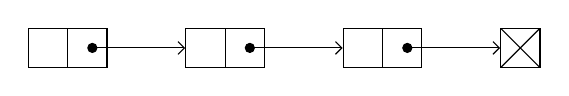
\begin{tikzpicture}[draw, minimum width=0.5cm, minimum height=0.5cm]
    \node[draw] (h1) at (0, 0) {};
    \node[draw] (t1) at (0.5, 0) {};

    \node[draw] (h2) at (2, 0) {};
    \node[draw] (t2) at (2.5, 0) {};

    \node[draw] (h3) at (4, 0) {};
    \node[draw] (t3) at (4.5, 0) {};

    \node[draw] (e) at (6, 0) {};
    \path (e) pic {cross=0.35cm};

    \draw (t1.center) edge[{Circle[]}-{Straight Barb[]}] (h2);
    \draw (t2.center) edge[{Circle[]}-{Straight Barb[]}] (h3);
    \draw (t3.center) edge[{Circle[]}-{Straight Barb[]}] (e);
\end{tikzpicture}
\end{center}

\Ex

Binarno drevo je \textbf{ali} vozlišče, ki vsebuje levega otroka \textbf{in} vrednost \textbf{in} desnega otroka, \textbf{ali} list.

\begin{center}
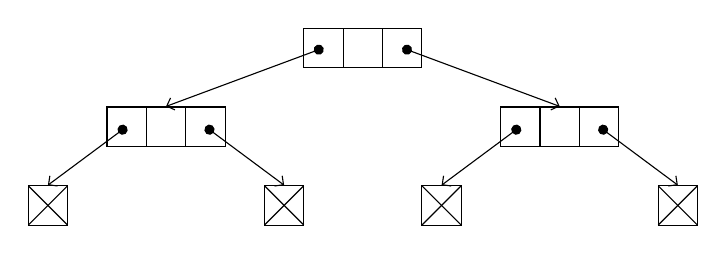
\begin{tikzpicture}[draw, minimum width=0.5cm, minimum height=0.5cm]
    \node[draw] (l1) at (-0.5, 0) {};
    \node[draw] (v1) at (0, 0) {};
    \node[draw] (r1) at (0.5, 0) {};

    \node[draw] (l2) at (-3, -1) {};
    \node[draw] (v2) at (-2.5, -1) {};
    \node[draw] (r2) at (-2, -1) {};

    \node[draw] (l3) at (2, -1) {};
    \node[draw] (v3) at (2.5, -1) {};
    \node[draw] (r3) at (3, -1) {};

    \node[draw] (e1) at (-4, -2) {};
    \node[draw] (e2) at (-1, -2) {};

    \node[draw] (e3) at (4, -2) {};
    \node[draw] (e4) at (1, -2) {};
    \path (e1) pic {cross=0.35cm};
    \path (e2) pic {cross=0.35cm};
    \path (e3) pic {cross=0.35cm};
    \path (e4) pic {cross=0.35cm};

    \draw (l1.center) edge[{Circle[]}-{Straight Barb[]}] (v2.north);
    \draw (r1.center) edge[{Circle[]}-{Straight Barb[]}] (v3.north);
    \draw (l2.center) edge[{Circle[]}-{Straight Barb[]}] (e1.north);
    \draw (r2.center) edge[{Circle[]}-{Straight Barb[]}] (e2.north);
    \draw (l3.center) edge[{Circle[]}-{Straight Barb[]}] (e4.north);
    \draw (r3.center) edge[{Circle[]}-{Straight Barb[]}] (e3.north);
\end{tikzpicture}
\end{center}

V modernih OOP jezikih obstaja implementacija $0$, ki se imenuje \emph{Void}, in implementacija $1$, ki se imenuje \emph{Unit}.
\emph{Void} ni enak ključni besedi \texttt{void} iz C++, \texttt{void} je v resnici \emph{Unit}!
Razlog je, da procedure ne morejo vračati nič, saj ne moremo ustvariti primerka nič, ker nič ne obstaja.
Lahko pa vračajo enoto, ta ima en sam primerek.
Če ta obrazložitev zveni preveč filozofsko, se spomnite, da je $0$ prazna množica in $1$ množica z enim elementom.

V funkcijskih jezikih operacijo ${(\Seq)}$ predstavimo kot tuple ali record in operacijo ${(\Sum)}$ kot označeno unijo.
Mogoče pa ju je implementirati tudi izključno z uporabo funkcij (Church encoding).

V C++ lahko uporabimo OOP implementacijo ali operacijo ${(\Seq)}$ predstavimo kot \texttt{struct} in operacijo ${(\Sum)}$ kot kombinacijo \texttt{union} in oznake (torej implementiramo označeno unijo).
V novejših standardih, implementacija označene unije že obstaja v standardni knjižnici \texttt{std::variant}.

\section{Abstraktno sintaktično drevo}
Za vsak programski jezik obstaja "naravna" gramatika, ki pa je zaradi omejitev razčlenjevalnikov pogosto ne moremo direktno uporabiti.
Če to "naravno" gramatiko pretvorimo v podatkoven tip dobimo abstraktno sintaktično drevo (AST).

\Ex
\begin{equation*}
  \begin{aligned}[t]
    \NT{Numbers} \Arrow \T{num} \Spc \NT{Numbers} \Union \Null\\[1em]
    \T{num} = \KleenePlus{\{\Char{0}, \dots, \Char{9}\}}
  \end{aligned}
  \qquad
  \begin{aligned}[t]
    Numbers &= Num \Seq Numbers \Sum 1\\
    Num &= Int\\
    Int &= 2^{32}\\
    Numbers &= List(Int)
  \end{aligned}
\end{equation*}
Pretvorba je 1:1, samo zamenjamo operacije.
Za terminale, če je mogoče, uporabimo vgrajene tipe, čeprav določenih leksemov ne bo mogoče pretvoriti v ta podatkovni tip.

\Ex
\begin{equation*}
  \begin{aligned}[t]
    \NT{Expr} &\Arrow \NT{Expr} \Spc \T{plus} \Spc \NT{Expr} \\
    &\Union \NT{Expr} \Spc \T{minus} \Spc \NT{Expr} \\
    &\Union \T{num}\\
    &\Union \T{var}\\[1em]
    \T{num} &= \KleenePlus{\{\Char{0}, \dots, \Char{9}\}}\\
    \T{char} &= \{\Char{A}, \dots, \Char{Z}, \Char{a}, \dots, \Char{z}, \Char{0}, \dots, \Char{9} \}\\
    \T{var} &= \KleenePlus{\T{char}}\\
    \T{plus} &= \Char{+}\\
    \T{minus} &= \Char{-}\\
  \end{aligned}
  \qquad
  \begin{aligned}[t]
    Expr &= Expr \Seq Plus \Seq Expr \\
    &\Sum Expr \Seq Minus \Seq Expr \\
    &\Sum Num\\
    &\Sum Var\\
    Num &= Int\\
    Var &= String\\
    Plus &= 1\\
    Minus &= 1\\[1em]
    Expr &= Expr \Seq Expr \\
    &\Sum Expr \Seq Expr \\
    &\Sum Int\\
    &\Sum Var
  \end{aligned}
\end{equation*}
Opazite, da imata $\T{plus}$ in $\T{minus}$ samo eno možno vrednost, torej sta izomorfna $1$.
Zato ju lahko izpustimo iz AST.
Izrazi so zelo podobni binarnim drevesom, le da imamo različno vrsto vozlišča za vsako operacijo.

\Ex
\begin{equation*}
  \begin{aligned}[t]
    \NT{Stmt} &\Arrow \NT{Var} \Spc \T{assign} \Spc \NT{Expr} \NT{Stmt}\\
    &\Union \T{print} \Seq \NT{Expr} \Spc \NT{Stmt}\\
    &\Union \Null\\[1em]
    \T{char} &= \{\Char{A}, \dots, \Char{Z}, \Char{a}, \dots, \Char{z}, \Char{0}, \dots, \Char{9} \}\\
    \T{var} &= \KleenePlus{\T{char}}\\
    \T{assign} &= \Char{=}\\
    \T{semi} &= \Char{;}\\
    \T{print} &= \Char{print}\\
  \end{aligned}
  \qquad
  \begin{aligned}[t]
    Stmt &= Var \Seq Assign \Seq Expr \Seq Stmt \\
    &\Sum Print \Seq Expr \Seq Stmt \\
    &\Sum 1\\
    Var &= String\\
    Assign &= 1\\
    Semi &= 1\\
    Print &= 1\\[1em]
    Stmt &= Var \Seq Expr \Seq Stmt \\
    &\Sum Expr \Seq Stmt \\
    &\Sum 1\\
  \end{aligned}
\end{equation*}
Izjave so zelo podobne seznamom, le da imamo različno vrsto celice za vsak ukaz.

\section{Konkretno sintaktično drevo}
Za razčlenjevanje moramo "naravno" gramatiko preoblikovati.
Če preoblikovano gramatiko pretvorimo v podatkoven tip dobimo konkretno sintaktično drevo (CST).
Ker je nadaljnje transformacije lažje izvesti nad AST, vedno najprej pretvorimo CST v AST.
Pretvorbo je mogoče izvesti kar med razčlenjevanjem (torej CST ne potrebujemo).

\chapter{Drevesne gramatike}
Podobno kot lahko imamo gramatike nad nizi, lahko imamo gramatike nad drevesi.
V primeru dreves so terminali vozlišča z $n$ otroci, za $n = 0, 1, 2 \dots$.

\Ex
\begin{equation*}
  \begin{aligned}
    List &\Arrow cell(Num, List) \Union end()\\
    Num &\Arrow int()\\[1em]
    List &\Derive cell(Num, List)\\
      &\Derive cell(int(), List)\\
      &\Derive cell(int(), cell(Num, List))\\
      &\Derive cell(int(), cell(int(), List))\\
      &\Derive cell(int(), cell(int(), cell(Num, List)))\\
      &\Derive cell(int(), cell(int(), cell(int(), end())))\\
  \end{aligned}
\end{equation*}

\Ex
\begin{equation*}
  \begin{aligned}
    Binary &\Arrow node(Binary, Num, Binary) \Union leaf()\\
    Num &\Arrow int()\\[1em]
    Binary &\Derive node(Binary, Num, Binary)\\
      &\Derive node(node(Binary, Num, Binary), Num, Binary)\\
      &\Derive node(node(leaf(), Num, Binary), Num, Binary)\\
      &\Derive node(node(leaf(), int(), Binary), Num, Binary)\\
      &\Derive node(node(leaf(), int(), leaf()), Num, Binary)\\
      &\Derive node(node(leaf(), int(), leaf()), int(), Binary)\\
      &\Derive node(node(leaf(), int(), leaf()), int(), node(Binary, Num, Binary))\\
      &\Derive node(node(leaf(), int(), leaf()), int(), node(leaf(), Num, Binary))\\
      &\Derive node(node(leaf(), int(), leaf()), int(), node(leaf(), int(), Binary))\\
      &\Derive node(node(leaf(), int(), leaf()), int(), node(leaf(), int(), leaf()))\\
  \end{aligned}
\end{equation*}

Algebraični podatkovni tipi \textbf{so} regularne drevesne gramatike.

Dovolimo lahko tudi vozlišča, ki imajo poljubno število otrok.
Torej otroci vozlišča spet tvorijo jezik.
Če se omejimo na regularne jezike jih lahko opišemo z regularnimi izrazi.
Primer takšnih dreves sta XML in sintaktična drevesa EBNF gramatik.

\Ex
\begin{equation*}
  \begin{aligned}
    Doc &\Arrow inventory(\Kleene{Item})\\
    Item &\Arrow desk(Desk) \Union chair(Chair) \Union computer(Computer) \\
    Info &\Arrow location(Location) \Seq \KleenePlus{user(User)}\\
    Location &\Arrow building(string()) \Seq room(Room)\\
    User &\Arrow name(Capitalized) \Seq surname(Capitalized) \Seq \Opt{role(Role)}\\
    Desk &\Arrow Info \Seq standing(boolean())\\
    Chair &\Arrow Info\\
    Computer &\Arrow Info \Seq cpu(Quantity) \Seq memory(Quantity) \Seq disk(Quantity)\\
    Capitalized &\Arrow string()\\
    Role &\Arrow string()\\
    Room &\Arrow integer()\\
    Quantity &\Arrow float()\\
  \end{aligned}
\end{equation*}
\newpage

\begin{lstlisting}
<inventory>
  <desk>
    <location>
      <building>G3</building>
      <room>13</room>
    </location>
    <user>
      <name>Albert</name>
      <surname>Einstein</surname>
      <role>Researcher</role>
    </user>
    <user>
      <name>Joe</name>
      <surname>Biden</surname>
    </user>
    <standing>false</standing>
  </desk>
  <computer>
    <location>
      <building>G3</building>
      <room>14</room>
    </location>
    <user>
      <name>Angelina</name>
      <surname>Jolie</surname>
      <role>Teacher</role>
    </user>
    <cpu>4.2</cpu>
    <memory>10.0</memory>
    <disk>10.0</disk>
  </computer>
  <chair>
    <location>
      <building>G3</building>
      <room>14</room>
    </location>
    <user>
      <name>Issac</name>
      <surname>Newton</surname>
      <role>Researcher</role>
    </user>
  </chair>
</inventory>
\end{lstlisting}

\printbibliography
\end{document}
